\documentclass[a4paper]{article}
\usepackage[14pt]{extsizes}
\usepackage[T2A]{fontenc}
\usepackage[T1]{fontenc}
\usepackage[utf8]{inputenc}
\usepackage[russian]{babel}
\usepackage{amsmath}
\usepackage[left=20mm, top=20mm, right=20mm, bottom=20mm, footskip=10mm]{geometry}
\usepackage{ragged2e}
\usepackage{setspace}
\usepackage{moreverb}
\usepackage{indentfirst} 
\usepackage{moreverb}
\usepackage{algorithm}
\usepackage[noend]{algpseudocode}
\usepackage[export]{adjustbox}
\usepackage{caption} %заголовки плавающих объектов
\usepackage{fixltx2e}
\usepackage{booktabs}
\usepackage{multirow}
\usepackage[table,xcdraw]{xcolor}
\usepackage{lipsum}
\usepackage{afterpage}
\renewcommand\verbatimtabsize{4\relax}
\renewcommand{\arraystretch}{1.4}
\usepackage[font=small, singlelinecheck=false, justification=centering, format=plain, labelsep=period]{caption} 
\usepackage{listings} 
\usepackage{rotating}
\usepackage{graphicx}
\usepackage{tabularx}
\setcounter{figure}{1}
\usepackage{minted}

\usepackage[%  
    colorlinks=true,
    pdfborder={0 0 0},
    linkcolor=blue
]{hyperref}

\usepackage{caption}
\DeclareCaptionFont{white}{\color{white}} 
\DeclareCaptionFormat{listing}{\colorbox{gray}{\parbox{\textwidth}{#1#2#3}}}
\captionsetup[lstlisting]{format=listing,labelfont=white,textfont=white}
\usepackage{adjustbox} 

\usepackage{xcolor} 
\usepackage{hyperref}
\usepackage{nccmath}
\usepackage{tikz}
\usepackage{wrapfig}
\usepackage{graphicx}
\usepackage{pdfpages}


\textheight=24cm 
\textwidth=16cm 
\oddsidemargin=0pt 
\topmargin=-1.5cm 
\parindent=24pt
\parskip=0pt 
\tolerance=2000 
\flushbottom 
\addto\captionsrussian{\def\refname{Список использованных источников}}

\begin{document}
\lstset{ %
language=C,                 % выбор языка для подсветки (здесь это С)
basicstyle=\small\sffamily, % размер и начертание шрифта для подсветки кода
numbers=left,               % где поставить нумерацию строк (слева\справа)
numberstyle=\tiny,           % размер шрифта для номеров строк
stepnumber=1,                   % размер шага между двумя номерами строк
numbersep=5pt,                % как далеко отстоят номера строк от подсвечиваемого кода
backgroundcolor=\color{white}, % цвет фона подсветки - используем \usepackage{color}
showspaces=false,            % показывать или нет пробелы специальными отступами
showstringspaces=false,      % показывать или нет пробелы в строках
showtabs=false,             % показывать или нет табуляцию в строках
frame=single,              % рисовать рамку вокруг кода
tabsize=2,                 % размер табуляции по умолчанию равен 2 пробелам
captionpos=t,              % позиция заголовка вверху [t] или внизу [b] 
breaklines=true,           % автоматически переносить строки (да\нет)
breakatwhitespace=false, % переносить строки только если есть пробел
escapeinside={\%*}{*)}   % если нужно добавить комментарии в коде
}

\lstloadlanguages{ [LaTeX] TeX}
% включаем кириллицу и добавляем кое−какие опции
\lstset{language =[LaTeX] TeX, % выбираем язык по умолчанию
	extendedchars=true , % включаем не латиницу
	escapechar = | , % |«выпадаем» в LATEX|
	frame=tb , % рамка сверху и снизу
	commentstyle=\itshape , % шрифт для комментариев
	%stringstyle =\bfseries,
        basicstyle=\tiny} % шрифт для строк
\lstset{
  literate={а}{{\selectfont\char224}}1
           {б}{{\selectfont\char225}}1
           {в}{{\selectfont\char226}}1
           {г}{{\selectfont\char227}}1
           {д}{{\selectfont\char228}}1
           {е}{{\selectfont\char229}}1
           {ё}{{\"e}}1
           {ж}{{\selectfont\char230}}1
           {з}{{\selectfont\char231}}1
           {и}{{\selectfont\char232}}1
           {й}{{\selectfont\char233}}1
           {к}{{\selectfont\char234}}1
           {л}{{\selectfont\char235}}1
           {м}{{\selectfont\char236}}1
           {н}{{\selectfont\char237}}1
           {о}{{\selectfont\char238}}1
           {п}{{\selectfont\char239}}1
           {р}{{\selectfont\char240}}1
           {с}{{\selectfont\char241}}1
           {т}{{\selectfont\char242}}1
           {у}{{\selectfont\char243}}1
           {ф}{{\selectfont\char244}}1
           {х}{{\selectfont\char245}}1
           {ц}{{\selectfont\char246}}1
           {ч}{{\selectfont\char247}}1
           {ш}{{\selectfont\char248}}1
           {щ}{{\selectfont\char249}}1
           {ъ}{{\selectfont\char250}}1
           {ы}{{\selectfont\char251}}1
           {ь}{{\selectfont\char252}}1
           {э}{{\selectfont\char253}}1
           {ю}{{\selectfont\char254}}1
           {я}{{\selectfont\char255}}1
           {А}{{\selectfont\char192}}1
           {Б}{{\selectfont\char193}}1
           {В}{{\selectfont\char194}}1
           {Г}{{\selectfont\char195}}1
           {Д}{{\selectfont\char196}}1
           {Е}{{\selectfont\char197}}1
           {Ё}{{\"E}}1
           {Ж}{{\selectfont\char198}}1
           {З}{{\selectfont\char199}}1
           {И}{{\selectfont\char200}}1
           {Й}{{\selectfont\char201}}1
           {К}{{\selectfont\char202}}1
           {Л}{{\selectfont\char203}}1
           {М}{{\selectfont\char204}}1
           {Н}{{\selectfont\char205}}1
           {О}{{\selectfont\char206}}1
           {П}{{\selectfont\char207}}1
           {Р}{{\selectfont\char208}}1
           {С}{{\selectfont\char209}}1
           {Т}{{\selectfont\char210}}1
           {У}{{\selectfont\char211}}1
           {Ф}{{\selectfont\char212}}1
           {Х}{{\selectfont\char213}}1
           {Ц}{{\selectfont\char214}}1
           {Ч}{{\selectfont\char215}}1
           {Ш}{{\selectfont\char216}}1
           {Щ}{{\selectfont\char217}}1
           {Ъ}{{\selectfont\char218}}1
           {Ы}{{\selectfont\char219}}1
           {Ь}{{\selectfont\char220}}1
           {Э}{{\selectfont\char221}}1
           {Ю}{{\selectfont\char222}}1
           {Я}{{\selectfont\char223}}1
}

\title{БД_отчет}
\author{Полина Радионова}


\includepdf{титул.pdf}
	
\setcounter{page}{2}
\newpage
\section*{Реферат}
Курсовая работа посвящена разработке базы данных для предметной области «Функционирование работы многопрофильной ветеринарной клиники», которая включает учёт ветеринаров, администраторов, клиентов и их питомцев, записи на приёмы, медицинские назначения и покупки в зоомагазине. Основная проблема заключалась в необходимости эффективного хранения и быстрого доступа к данным о животных, их владельцах и оказанных услугах. В ходе работы была проанализирована предметная область, спроектирована реляционная база данных, создана и заполнена база данных, а также был написан код для 8 запросов, сформированных на основе созданной базы данных. База данных была реализована в командной строке MySQL, взаимодействие с базой осуществлялось через консоль Windows. Для заполнения базы данных был написан программный код на языке Python. Полученная система может быть внедрена в ветеринарных клиниках для автоматизации учёта пациентов и упрощения работы администраторов.

\newpage
{\small \tableofcontents}

\newpage
\section*{Введение}
\addcontentsline{toc}{section}{Введение}
Современные организации ежедневно сталкиваются с необходимостью управления большими объемами информации. В условиях ручной обработки информации возрастают риски ошибок, потери данных и неэффективного использования времени сотрудников. Особенно остро эта проблема проявляется в сферах, где важны точность и оперативность обработки данных.

Система баз данных -- ключевой инструмент для структурирования информации и её обработки. Базу данных можно рассматривать как хранилище для значительно большого объема информации, занесенного в компьютер. 

Базы данных заменяют бумажные архивы и обеспечивают мгновенный доступ к данным. Они ускоряют процесс выполнения обычных операций, минимизируют дублирование и позволяют нескольким пользователям работать с информацией одновременно. Это может быть полезно для отслеживания множественных процессов работы ветеринарной клиники.

Основой взаимодействия с такими системами являются запросы на языке SQL. Запросы дают возможность гибко управлять данными: добавлять, удалять, сортировать и анализировать их в реальном времени. Язык SQL реализует выборку данных по заданным критериям независимо от обновления информации, хранящейся в базе данных.

При этом эффективное проектирование базы данных требует тщательного анализа предметной области и оптимизации структуры таблиц для минимизации избыточности информации. Грамотно спроектированная база данных не только обеспечивает целостность и безопасность данных, но и значительно повышает производительность работы всей информационной системы в целом.

\newpage
\section{Постановка задачи}
Цель: реализовать базу данных для предметной области <<Функционирование работы ветеринарной клиники>>.

Для достижения поставленной цели было выделено несколько задач.

\begin{enumerate}
    \item Составление описания предметной области и формулировка целей создания базы данных.
    \item Создание ER-диаграммы.
    \item Проектирование базы данных и её лингвистического и графического описания.
    \item Создание базы данных.
    \item Заполнение базы данных 200-300 тысячами значений.
    \item Написание 8 запросов на языке SQL.
    \item Генерация 3 гистограмм.
\end{enumerate}

\newpage
\section{Исследование процессов работы ветеринарной клиники}
\subsection{Описание предметной области}
Ветеринарная клиника — специализированное медицинское учреждение, которое оказывает врачебную помощь и обеспечивает уход за домашними животными.

Раннее ветеринария рассматривалась как отрасль общей медицины, однако сейчас она является областью научных знаний, предметом изучения которой является лечение болезней животных, производство безопасных для человека сельскохозяйственных продуктов и защита людей от зоонозных болезней  — заболеваний, общих для человека и животных.

Активный рост ветеринарной медицины в России был тесно связан с историческими потребностями. Вспышки инфекционных заболеваний среди животных, особенно лошадей, потребовали вмешательства: лошади играли важную роль в армии, транспорте и сельском хозяйстве, и их здоровье было необходимо для привычного функционирования государства \cite{vetmed}. Параллельно, развитие животноводства требовало квалифицированных специалистов для лечения сельскохозяйственного скота. Обеспечение здоровья скота напрямую влияло на продовольственные запасы. Таким образом, ветеринария стала неотъемлемой частью сельского хозяйства и национальной безопасности.

Со второй половины XX века произошел значительный сдвиг в отношении человека к животным.  Некоторые виды животных человек стал воспринимать не только в плоскости служебной или экономической ценности, но и как компаньонов для жизни. Сейчас все больше людей видят в своём питомце объект тёплого общения и внимания, способный давать хозяину радость и эмоции. Вторая половина 60-х годов XX века стала отправной точкой для формирования нового социально-культурного явления – признания за животными-компаньонами определенных прав и потребностей.
Возрастающая роль животных в жизни людей, особенно в качестве компаньонов, привела к активному развитию «зооиндустрии». К ней относятся услуги передержки, груминга, производство специализированных кормов, игрушек, одежды и аксессуаров. Это же и стало причиной возникновения ветеринарии мелких домашних животных (ВМДЖ) — области ветеринарной медицины, занимающаяся лечением и профилактикой заболеваний у животных-компаньонов: кошек, собак, попугаев, грызунов и многих других питомцев, содержащихся в квартирах. 
К середине 1980-х годов в Советском Союзе появилась отдельная специализация ветеринарных врачей, занимающихся лечением исключительно кошек и собак. В конце 1990-х — начале 2000-х годов в Москве и Санкт-Петербурге появились первые клиники со стационарным лечением, широким спектром аппаратной диагностики для животных. В этих центрах врачи уже имели специализацию.

В настоящие дни работа крупных центров, специализирующихся на помощи мелким домашним животным, не отличается от таковых в гуманитарной медицине \cite{gost}. Существуют экспертного уровня ветеринарные офтальмологи, кардиологи, хирурги, эндокринологи, дерматологи, стоматологи, аллергологи и специалисты всех других медицинских направлений. В клиниках для животных способны выполнять сложнейшие операции и диагностические исследования: ЭКГ, УЗИ, компьютерная томография, ренгенография, лабораторные анализы и многие другие. В последние годы все большее значение приобретает превентивная медицина, направленная на профилактику заболеваний с помощью вакцинации, правильного питания и регулярных осмотров.

Ветеринарные клиники также предлагают дополнительные услуги, включая ветеринарную аптеку, где можно приобрести необходимые лекарственные препараты, специальные корма и средства по уходу за питомцами. В случае, когда помочь животному уже невозможно, ветеринарные клиники предлагают услуги эвтаназии и кремации.

Работа ветеринарных клиник в целом похожа на работу обыкновенных частных клиник. Владелец животного может обратиться в любой понравившийся ему ветеринарный центр, зарегистрировать своего питомца и записать его на прием. Ветеринарный врач осмотрит животное, соберет анамнез, поставит первичный диагноз, даст свои комментарии и рекомендации по уходу и лечению и может даже дать направление к другому специалисту: например, кардиологу или аллергологу. После первого же приема у питомца появится своя медицинская карточка в этой клинике, в которой будет храниться вся основная информация о животном, история его обращений, результаты анализов и исследований, а также сведения о проведенных вакцинациях и лечении. Это позволяет ветеринарным врачам отслеживать состояние здоровья животного и оказывать ему наиболее эффективную и своевременную помощь.

В будущем можно ожидать дальнейшего развития ветеринарной медицины: уже сейчас производится трансплантация органов, активно развивается протезирование для животных.  После травм и операций осуществляется реабилитация для домашних питомцев, например, физиотерапия и гидротерапия. Все это делает ветеринарию не только наукой  о лечении, но и повышении качества жизни домашних животных. 

Несмотря на активный рост развития ветеринарной медицины в России и большую потребность в этом среди населения, государство не осуществляет участие в контроле вопросов, связанных с содержанием животных \cite{civilcode}. На данный момент отстутствуют стандарты оказания медицинской помощи домашним питомцам, система лицензирования ветеринарных клиник и сертификации врачей. Это создает определенные риски для владельцев животных, так как на рынке могут появляться неквалифицированные специалисты и недобросовестные клиники. Отсутствие финансирования государством ветеринарных услуг приводит к высокой стоимости лечения для владельцев животных. 

Таким образом, ветеринарная медицина прошла долгий путь развития – от надзора за заразными болезнями скота до высокотехнологичных центров, предлагающих полный спектр услуг для домашних питомцев. Однако в заключение стоит подчеркнуть, что здоровье домашнего питомца – это всегда ответственность его владельца.

\subsection {Цели создания базы данных}
\begin{enumerate}
	\item Хранение клиентской карточки хозяина животного.
	\item Хранение медицинской карточки питомца.
	\item Хранение информации о персонале.
	\item Хранение информации о проданных товарах.
\end{enumerate}

\subsection {Описание сущностей}
\begin{enumerate}
\item Ветеринарная клиника -- медицинкое учреждение, специализирующееся на оказании врачебной помощи домашним животным.

Атрибуты: адрес, номер телефона.

\item Администратор -- специалист, общающийся с клиентами клиники, координирующий расписание приемов и осуществляющий продажу лекарственных препаратов, кормов и других ветеринарных средств. 

Атрибуты: ФИО, номер телефона, адрес электронной почты.

\item Ветеринар -- врач, специализирующийся на уходе и лечении мелких домашних животных. 

Атрибуты: ФИО, специализация, квалификация, адрес проживания, адрес электронной почты, номер телефона. 

\item Медицинский приём -- комплекс мероприятий, включающий в себя сбор анамнеза, осмотр, проведение диагностических процедур или медицинских услуг, постановку диагноза и назначение лечения.

Атрибуты: статус приёма, причина обращения, предоставленная услуга, заключение, назначение.

\item Питомец -- домашнее животное, имеющее владельца.

Атрибуты: кличка, дата рождения, пол, вид, порода, номер чипа, аллергия.

\item Владелец питомца -- человек, содержащий у себя дома животное.

Атрибуты: ФИО, номер телефона, адрес электронной почты, адрес проживания.

\item Товар -- ветеринарное средство, продаваемое в ветеринарной клинике.

Атрибуты: наименование, страна производства, поставщик, цена.
\end{enumerate}

\subsection {Описание ролей}
\textit{Администратор} является работником ветеринарной клиники и играет роль связующего звена между владельцем питомца и ветеринарным врачом. Он общается с клиентами, осуществляет их запись к врачу, напоминает им о приемах и осуществляет оплату оказанных медицинских услуг. Администратор также производит продажу лекарственных препаратов, кормов и других ветеринарных средств, вплоть до игрушек для животных.

\textit{Владелец питомца} обращается в ветеринарную клинику очно или онлайн и  через администратора запиывает своего питомца на прием. Он оплачивает оказанные питомцу медицинские услуги и покупает товары в ветеринарной аптеке.

\textit{Ветеринар} является лечащим специалистом ветеринарной клиники и проводит медицинские приемы согласно своему расписанию. Он собирает анамнез, проводит осмотр, оказывает медицинские услуги, ставит диагноз и дает назначения и рекомендации к лечению.

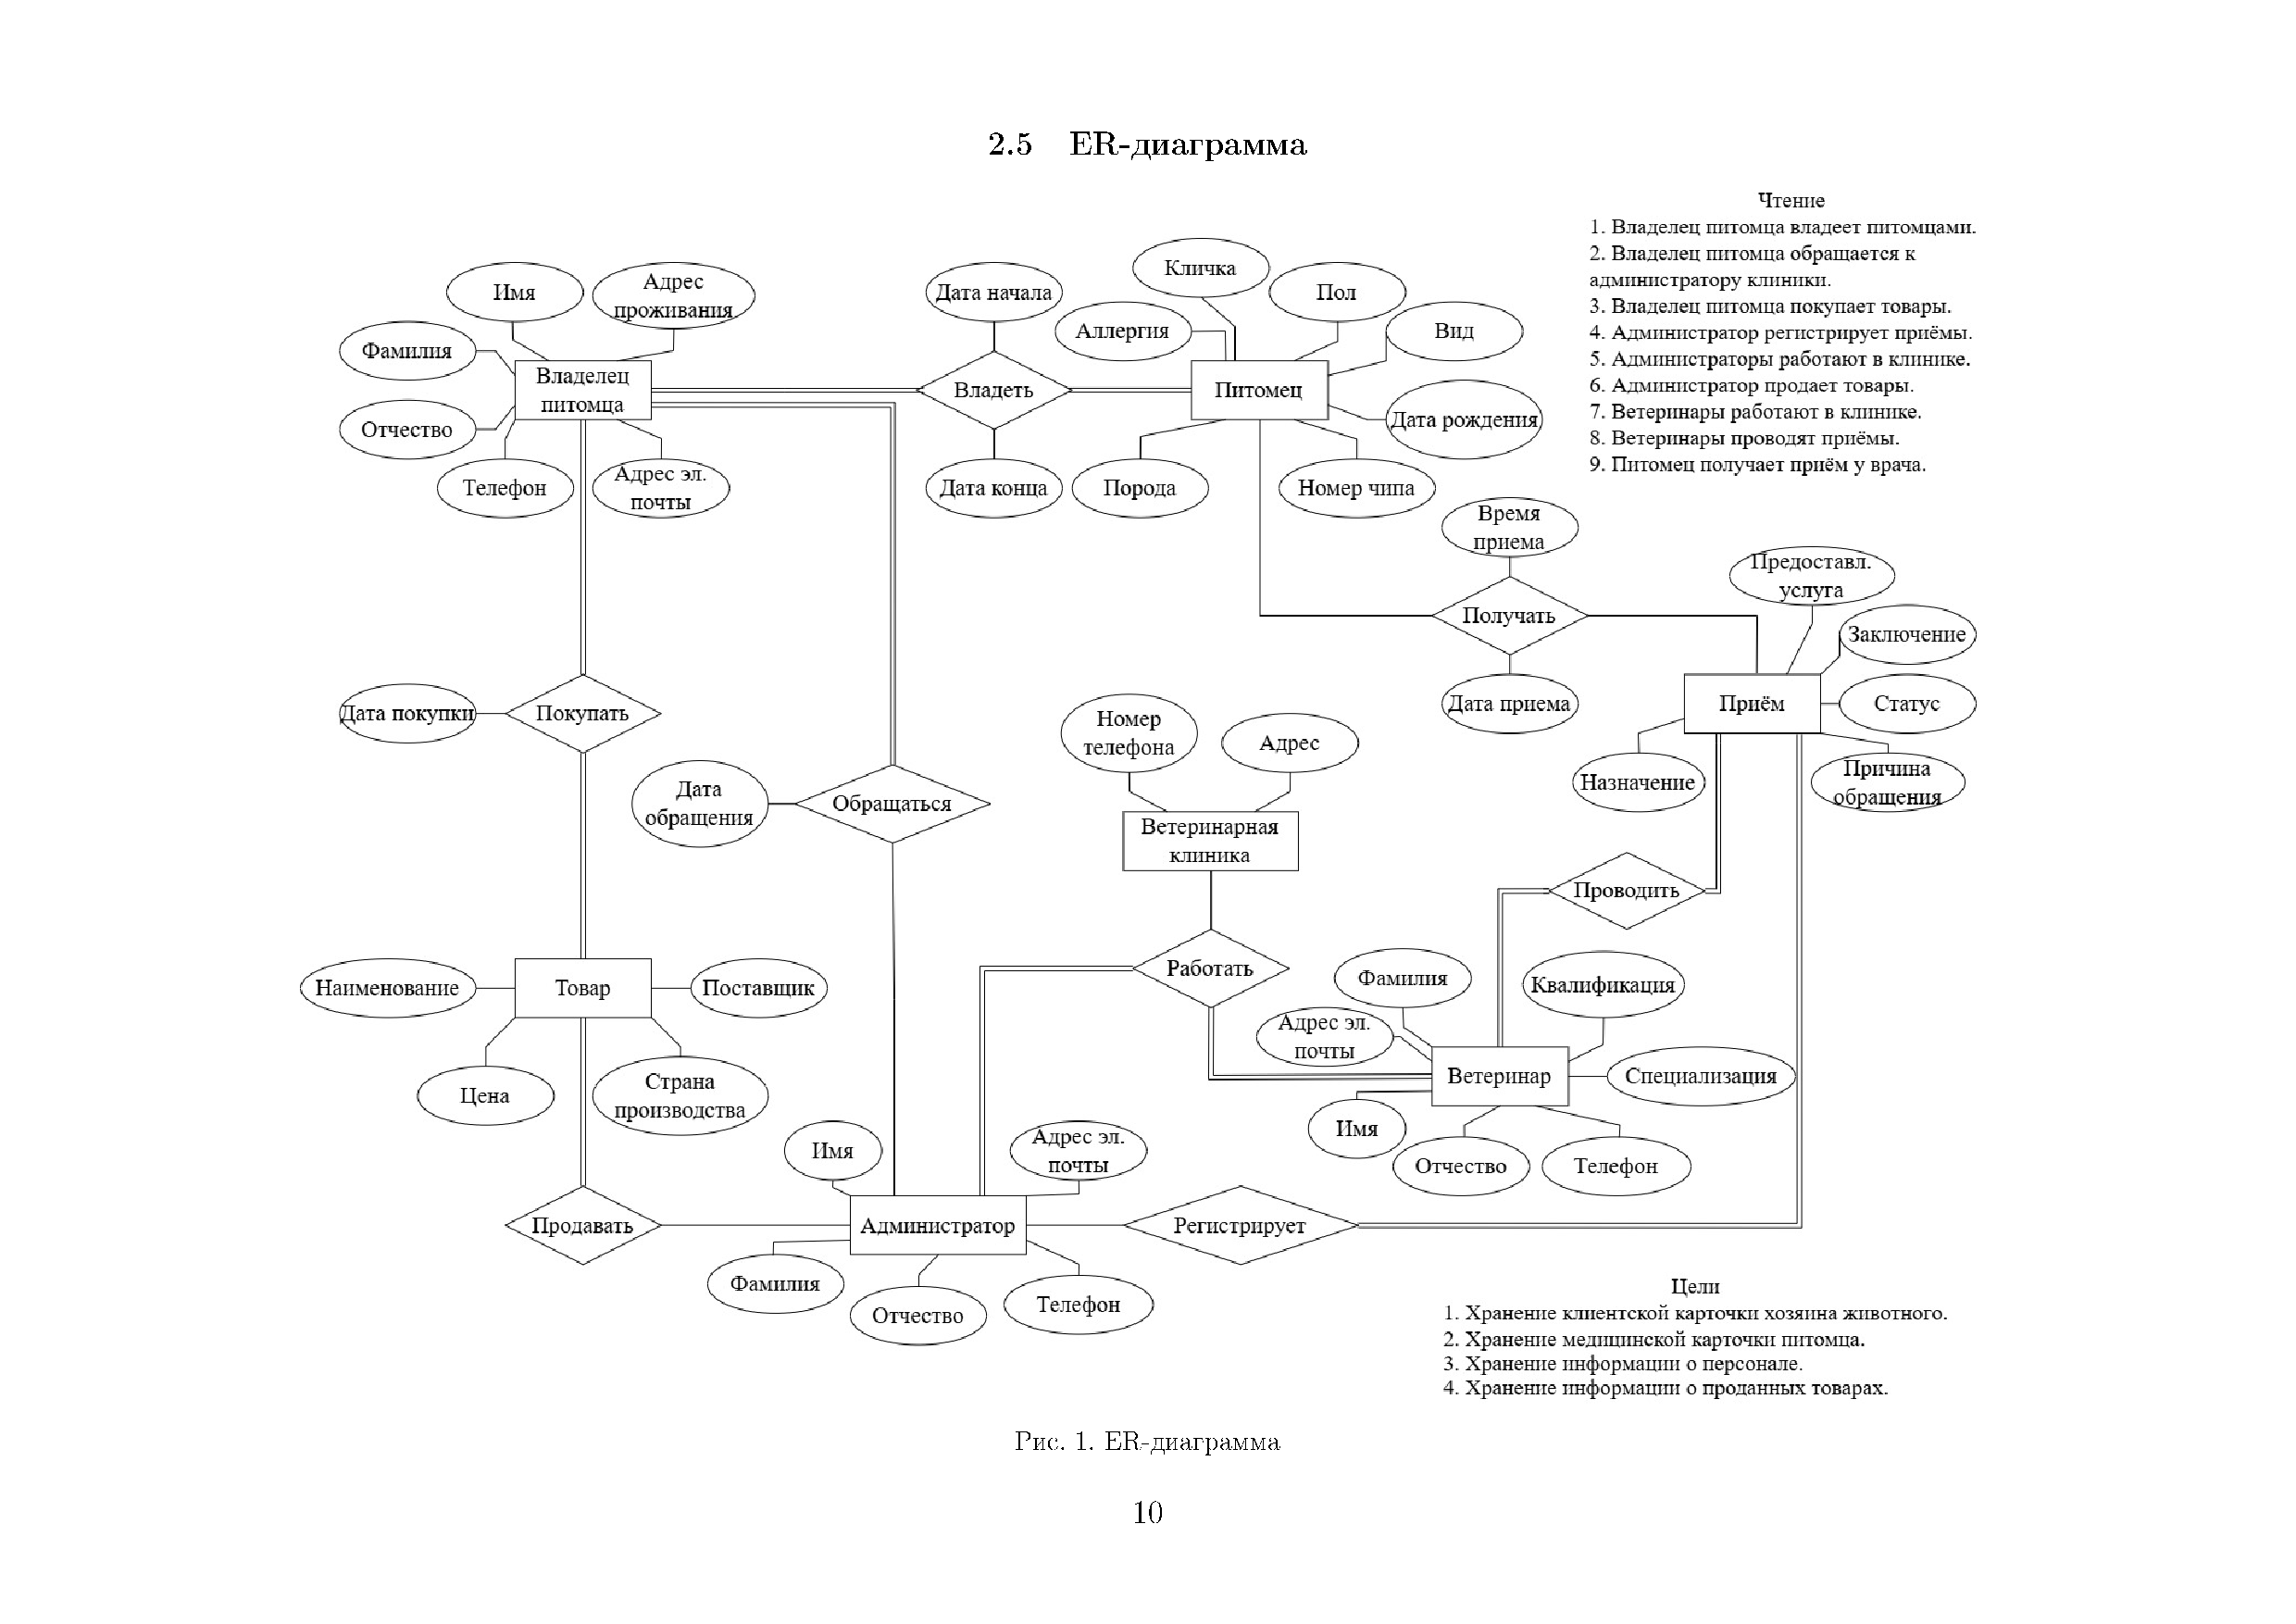
\includepdf[fitpaper]{er.pdf}
\addcontentsline{toc}{subsection}{2.5 \hspace{0.35cm}ER-диаграмма} 

\setcounter{subsection}{5}
\subsection {Чтение ER-диаграммы}
ER-диаграмма приведена на рис. 1.
\begin{enumerate}
\item Владелец питомца владеет питомцами.

\item Владелец питомца обращается к администратору клиники.

\item Владелец питомца покупает товары.

\item Администратор регистрирует приёмы.

\item Администраторы работают в клинике.

\item Администратор продает товары.

\item Ветеринары работают в клинике. 

\item Ветеринары проводят приёмы. 

\item Питомец получает приём у врача.
\end{enumerate}

\subsection {Схема связи объектов}
На рис. \ref{shema} представлена схема связи объектов базы данных.

\begin{figure}[h!]
\begin{center}
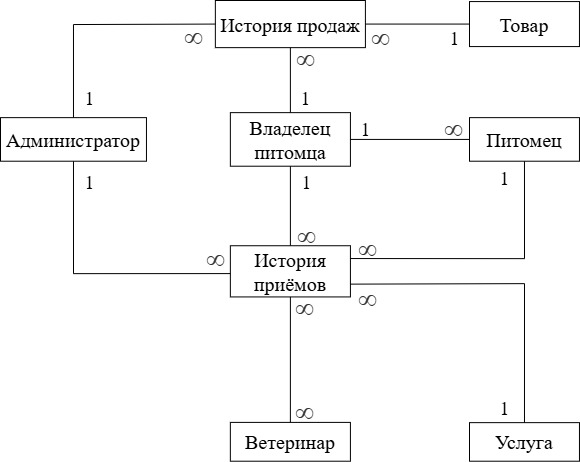
\includegraphics[width=11cm]{shema.jpg}
\captionsetup{justification=centering}
\caption{Схема связи объектов}
\label{shema}
\centering
\end{center}
\end{figure}

\newpage
\section{Проектирование}
\subsection{Таблицы с описанием таблиц баз данных}
В таблицах 1-12 описаны атрибуты каждой таблицы проектирумой базы данных. В таблицах перечислены: признак ключа, если поле является ключом, имя атрибута на русском и на английском языках, тип атрибута, размер переменной, значение атрибута по умолчанию. Для внешних ключей также указаны ссылки на таблицы и атрибуты первичных ключей. 

Ограничение в 14 символов для атрибута <<Вид\_название>> в таблице \ref{tab:Вид} обусловлено тем, что это максимальное количество символов среди всех имеющихся в предметной области видов мелких домашних животных. 

\begin{table}[H]
  \caption{Вид - species}
  \resizebox{\columnwidth}{!}{%
     \begin{tabular}{|c|c|c|c|c|c|c|}
      \hline
      \multicolumn{7}{|c|}{Вид - species}\\
      \cline{1-7}
      №&Тип ключа&Название RU&Название EN&Тип атрибута&NULL/NOT NULL&Ссылка\\
      \cline{1-7}
      1 & PK & Вид\_id & species\_id & INT & NOT NULL & - \\
      2 & - & Вид\_название & name & VARCHAR(14) & NOT NULL & -\\
      \hline
    \end{tabular}\mbox{} 
  }
  \label{tab:Вид}
\end{table}

Ограничение в 40 символов для атрибута <<Порода\_название>> в таблице \ref{tab:Порода} обусловлено количеством символов в самом длинном названии породы в предметной области. 

\begin{table}[H]
  \caption{Порода - breed}
  \resizebox{\columnwidth}{!}{
     \begin{tabular}{|c|c|c|c|c|c|c|}
      \hline
      \multicolumn{7}{|c|}{Порода - breed}\\
      \cline{1-7}
      №&Тип ключа&Название RU&Название EN&Тип атрибута&NULL/NOT NULL&Ссылка\\
      \cline{1-7}
      1 & PK & Порода\_id & breed\_id & INT & NOT NULL & - \\
      2 & - & Порода\_название & name & VARCHAR(40) & NOT NULL & -\\
      3 & FK & Вид\_id & species\_id & INT & NOT NULL & species(species\_id)\\
      \hline
    \end{tabular}\mbox{} 
  }
  \label{tab:Порода}
\end{table}

Ограничение в 50 символов для атрибутов <<Владелец\_имя>>, <<Владелец\_фамилия>> и <<Владелец\_отчество>> в таблице \ref{tab:Владелец} обусловлено тем, что в среднем их длина в выбранной библиотеке Python.Faker не превышает 47 символов. 

Ограничение в 20 символов для атрибута <<Владелец\_номер\_телефо-на>> в таблице \ref{tab:Владелец} установлено для возможности использовать символы-разделители, такие как скобка и дефис, совместно с 11 цифрами номера телефона.

Ограничение в 254 символа для атрибута <<Владелец\_адрес\_эл\_поч-ты>> в таблице \ref{tab:Владелец} обусловлено тем, что максимальная длина адреса электронной почты составляет 254 символа. 

Ограничение в 100 символов для атрибута <<Владелец\_адрес\_прожи-вания>> в таблице \ref{tab:Владелец} обусловлен тем, что самый длинный адрес из списка содержит 96 символов. 

\begin{table}[H]
  \caption{Владелец - owner}
  \resizebox{\columnwidth}{!}{%
     \begin{tabular}{|c|c|c|c|c|c|c|}
      \hline
      \multicolumn{7}{|c|}{Владелец - owner}\\
      \cline{1-7}
      №&Тип ключа&Название RU&Название EN&Тип атрибута&NULL/NOT NULL&Ссылка\\
      \cline{1-7}
      1 & PK & Владелец\_id & vet\_id & INT & NOT NULL & - \\
      2 & - & Владелец\_имя & first\_name & VARCHAR(50) & NOT NULL & -\\
      3 & - & Владелец\_фамилия & second\_name & VARCHAR(50) & NOT NULL & -\\
      4 & - & Владелец\_отчество & middle\_name & VARCHAR(50) & NULL & -\\
      5 & - & Владелец\_номер\_телефона & phone\_number & VARCHAR(20) & NOT NULL & -\\
      6 & - & Владелец\_адрес\_эл\_почты & email & VARCHAR(254) & NULL & -\\
      7 & - & Владелец\_адрес\_проживания & address & VARCHAR(100) & NULL & -\\
      \hline
    \end{tabular}\mbox{} 
  }
  \label{tab:Владелец}
\end{table}

Ограничение в 50 символов для атрибута <<Питомец\_кличка>> в таблице \ref{tab:Питомец} установлено потому, что в среднем самые длинные клички выставочных животных не превышают 50 символов. 

Ограничение в 7 символов для атрибута <<Питомец\_пол>> в таблице \ref{tab:Питомец} обусловлено максимальным количеством символов среди возможных значений <<Male>> и <<Female>>.

Ограничение в 100 символов для атрибута <<Питомец\_аллергия>> в таблице \ref{tab:Питомец} установлено потому, что у питомца может быть несколько аллергий, объединенных в одну строку и перечисленных через запятую или точку с запятой.

\begin{table}[H]
  \caption{Питомец - pet}
  \resizebox{\columnwidth}{!}{%
     \begin{tabular}{|c|c|c|c|c|c|c|}
      \hline
      \multicolumn{7}{|c|}{Питомец - pet}\\
      \cline{1-7}
      №&Тип ключа&Название RU&Название EN&Тип атрибута&NULL/NOT NULL&Ссылка\\
      \cline{1-7}
      1 & PK & Питомец\_id & vet\_id & INT & NOT NULL & - \\
      2 & - & Питомец\_кличка & nickname & VARCHAR(50) & NOT NULL & -\\
      3 & - & Питомец\_дата\_рождения & birth\_date & DATE & NULL & -\\
      4 & - & Питомец\_пол & sex & VARCHAR(7) & NOT NULL & -\\
      5 & - & Питомец\_аллергия & allergy & VARCHAR(100) & NULL & -\\
      6 & - & Питомец\_номер\_чипа & chip\_number & INT & NULL & -\\
      7 & FK & Владелец\_id & owner\_id & INT & NOT NULL & owner(owner\_id)\\
      8 & FK & Вид\_id & species\_id & INT & NOT NULL & species(species\_id)\\
      9 & FK & Порода\_id & breed\_id & INT & NULL & breed(breed\_id)\\
      \hline
    \end{tabular}\mbox{} 
  }
  \label{tab:Питомец}
\end{table}

Ограничение в 30 символов для атрибута <<Услуга\_название>> в таблице \ref{tab:Услуга} обусловлено тем, что самое длинное название в таблице составляет 28 символов. 

Ограничение в 10 символов для атрибута <<Услуга\_цена>> в таблице \ref{tab:Услуга} обусловлено тем, что максимальная стоимость из списка (<<10 000>>) состоит из 6 символов.

\begin{table}[H]
  \caption{Услуга - service}
  \resizebox{\columnwidth}{!}{%
     \begin{tabular}{|c|c|c|c|c|c|c|}
      \hline
      \multicolumn{7}{|c|}{Услуга - service}\\
      \cline{1-7}
      №&Тип ключа&Название RU&Название EN&Тип атрибута&NULL/NOT NULL&Ссылка\\
      \cline{1-7}
      1 & PK & Услуга\_id & service\_id & INT & NOT NULL & - \\
      2 & - & Услуга\_название & name & VARCHAR(30) & NOT NULL & -\\
      3 & - & Услуга\_цена & price & DECIMAL(10, 2) & NOT NULL & -\\
      \hline
    \end{tabular}\mbox{} 
  }
  \label{tab:Услуга}
\end{table}

Ограничение в 50 символов для атрибутов <<Администратор\_имя>>, <<Администратор\_фамилия>> и <<Администратор\_отчество>> в таблице \ref{tab:Админ} обусловлено тем, что в среднем их длина в выбранной библиотеке Python.Faker не превышает 47 символов. 

Ограничение в 20 символов для атрибута <<Администратор\_номер\_-телефона>> в таблице \ref{tab:Админ} установлено для возможности использовать символы-разделители, такие как скобка и дефис, совместно с 11 цифрами номера телефона.

Ограничение в 254 символа для атрибута <<Администратор\_адрес\_эл-поч-ты>> в таблице \ref{tab:Админ} обусловлено тем, что максимальная длина адреса электронной почты составляет 254 символа. 

\begin{table}[H]
  \caption{Администратор - administrator}
  \resizebox{\columnwidth}{!}{%
     \begin{tabular}{|c|c|c|c|c|c|c|}
      \hline
      \multicolumn{7}{|c|}{Администратор - administrator}\\
      \cline{1-7}
      №&Тип ключа&Название RU&Название EN&Тип атрибута&NULL/NOT NULL&Ссылка\\
      \cline{1-7}
      1 & PK & Администратор\_id & admin\_id & INT & NOT NULL & - \\
      2 & - & Администратор\_имя & first\_name & VARCHAR(50) & NOT NULL & -\\
      3 & - & Администратор\_фамилия & second\_name & VARCHAR(50) & NOT NULL & -\\
      4 & - & Администратор\_отчество & middle\_name & VARCHAR(50) & NOT NULL & -\\
      5 & - & Администратор\_номер\_телефона & phone\_number & VARCHAR(20) & NOT NULL & -\\
      6 & - & Администратор\_адрес\_эл\_почты & email & VARCHAR(254) & NOT NULL & -\\
      \hline
    \end{tabular}\mbox{} 
  }
  \label{tab:Админ}
\end{table}

Ограничение в 10 символов для атрибута <<Прием\_статус>> в таблице \ref{tab:Прием} установлен потому, что максимальная длина среди возможных значений: <<Completed>>, <<Cancelled>>, <<No-show>> -- составляет 9 символов.

Ограничение в 100 символов для атрибута <<Прием\_причина\_обраще-ния>> в таблице \ref{tab:Прием} установлено потому, что может быть названо несколько причин, объединенных в одну строку и перечисленных через запятую или точку с запятой.

Ограничение в 200 символов для атрибута <<Прием\_заключение>> в таблице \ref{tab:Прием} установлено потому, что ветеринар может поставить сразу несколько диагнозов, которые будут объединены в одну строку и перечислены через запятую или точку с запятой.

Ограничение в 200 символов для атрибута <<Прием\_назначение>> в таблице \ref{tab:Прием} установлено потому, что ветеринар может назначить лечение, состоящее из нескольких рекомендаций, которые будут объединены в одну строку и перечислены через запятую или точку с запятой.

\begin{table}[H]
  \caption{Прием - appointment}
  \resizebox{\columnwidth}{!}{%
     \begin{tabular}{|c|c|c|c|c|c|c|}
      \hline
      \multicolumn{7}{|c|}{Прием - appointment}\\
      \cline{1-7}
      №&Тип ключа&Название RU&Название EN&Тип атрибута&NULL/NOT NULL&Ссылка\\
      \cline{1-7}
      1 & PK & Прием\_id & appointment\_id & INT & NOT NULL & - \\
      2 & - & Прием\_статус & status & VARCHAR(10) & NOT NULL & -\\
      3 & - & Прием\_дата & appointment\_date & DATE & NULL & -\\
      4 & - & Прием\_время & appointment\_time & TIME & NOT NULL & -\\
      5 & - & Прием\_причина\_обращения & reason & VARCHAR(100) & NOT NULL & -\\
      6 & - & Прием\_заключение & conclusion & VARCHAR(200) & NULL & -\\
      7 & - & Прием\_назначение & treatment & VARCHAR(200) & NULL & -\\
      8 & FK & Услуга\_id & service\_id & INT & NOT NULL & service(service\_id)\\
      9 & FK & Питомец\_id & pet\_id & INT & NOT NULL & pet(pet\_id)\\
      10 & FK & Владелец\_id & owner\_id & INT & NOT NULL & owner(owner\_id)\\
      11 & FK & Администратор\_id & admin\_id & INT & NOT NULL & admin(admin\_id)\\
      \hline
    \end{tabular}\mbox{} 
  }
  \label{tab:Прием}
\end{table}

Ограничение в 50 символов для атрибутов <<Ветеринар\_имя>>, <<Ветеринар\_фамилия>> и <<Ветеринар\_отчество>> в таблице \ref{tab:Ветеринар} обусловлено тем, что в среднем их длина в выбранной библиотеке Python.Faker не превышает 47 символов. 

Ограничение в 20 символов для атрибута <<Ветеринар\_номер\_телефо-на>> в таблице \ref{tab:Ветеринар} установлено для возможности использовать символы-разделители, такие как скобка и дефис, совместно с 11 цифрами номера телефона.

Ограничение в 254 символа для атрибута <<Ветеринар\_адрес\_эл\_по-чты>> в таблице \ref{tab:Ветеринар} обусловлено тем, что максимальная длина адреса электронной почты составляет 254 символа. 

Ограничение в 15 символов атрибута <<Ветеринар\_специализация>> в таблице \ref{tab:Ветеринар} обусловлено тем, что слово максимальной длины среди возможных значений предметной области содержит 11 символов.

Ограничение в 6 символов атрибута <<Ветеринар\_квалификация>> в таблице \ref{tab:Ветеринар} обусловлено тем, что все возможные значения атрибута: <<высшая>>, <<первая>>, <<вторая>> -- содержат в себе 6 символов.

\begin{table}[H]
  \caption{Ветеринар - veterinarians}
  \resizebox{\columnwidth}{!}{%
     \begin{tabular}{|c|c|c|c|c|c|c|}
      \hline
      \multicolumn{7}{|c|}{Ветеринар - veterinarian}\\
      \cline{1-7}
      №&Тип ключа&Название RU&Название EN&Тип атрибута&NULL/NOT NULL&Ссылка\\
      \cline{1-7}
      1 & PK & Ветеринар\_id & vet\_id & INT & NOT NULL & - \\
      2 & - & Ветеринар\_имя & first\_name & VARCHAR(50) & NOT NULL & -\\
      3 & - & Ветеринар\_фамилия & second\_name & VARCHAR(50) & NOT NULL & -\\
      4 & - & Ветеринар\_отчество & middle\_name & VARCHAR(50) & NOT NULL & -\\
      5 & - & Ветеринар\_номер\_телефона & phone\_number & VARCHAR(20) & NOT NULL & -\\
      6 & - & Ветеринар\_адрес\_эл\_почты & email & VARCHAR(254) & NOT NULL & -\\
      7 & - & Ветеринар\_специализация & specialization & VARCHAR(15) & NOT NULL & -\\
      8 & - & Ветеринар\_квалификация & qualification & VARCHAR(6) & NOT NULL & -\\
      \hline
    \end{tabular}\mbox{} 
  }
  \label{tab:Ветеринар}
\end{table}

\begin{table}[H]
  \caption{Приемы и ветеринары - veterinarian and appointment}
  \resizebox{\columnwidth}{!}{%
     \begin{tabular}{|c|c|c|c|c|c|c|}
      \hline
      \multicolumn{7}{|c|}{Приемы и ветеринары - veterinarian and appointment}\\
      \cline{1-7}
      №&Тип ключа&Название RU&Название EN&Тип атрибута&NULL/NOT NULL&Ссылка\\
      \cline{1-7}
      1 & PK & Ветеринар\_прием\_id & vet\_app\_id & INT & NOT NULL & - \\
      2 & FK & Прием\_id & appointment\_id & INT & NOT NULL & appointment(appointment\_id)\\
      3 & FK & Ветеринар\_id & vet\_id & INT & NOT NULL & veterinarian(vet\_id)\\
      \hline
    \end{tabular}\mbox{} 
  }
  \label{tab:vandapp}
\end{table}

Ограничение в 50 символов у атрибута <<Поставщик\_имя>> в таблице \ref{tab:Поставщик} обусловлено тем, что в среднем длина названий компаний в выбранной библиотеке Python.Faker не превышает 50 символов. 

\begin{table}[H]
  \caption{Поставщик - supplier}
  \resizebox{\columnwidth}{!}{%
     \begin{tabular}{|c|c|c|c|c|c|c|}
      \hline
      \multicolumn{7}{|c|}{Поставщик - supplier}\\
      \cline{1-7}
      №&Тип ключа&Название RU&Название EN&Тип атрибута&NULL/NOT NULL&Ссылка\\
      \cline{1-7}
      1 & PK & Поставщик\_id & supplier\_id & INT & NOT NULL & -\\
      2 & - & Поставщик\_имя & name & VARCHAR(50) & NOT NULL & -\\
      \hline
    \end{tabular}\mbox{} 
  }
  \label{tab:Поставщик}
\end{table}

Ограничение в 50 символов у атрибута <<Товар\_наименование>> в таблице \ref{tab:Товар} обусловлено тем, что название товара может содержать в себе некоторые характеристики товара, такие как цвет или вкус. 

Ограничение в 20 символов у атрибута <<Товар\_страна\_производства>> в таблице \ref{tab:Товар} обусловлено тем, что очень длинные названия стран можно сократить до аббревиатуры, и в среднем названия стран не содержат в себе более 20 символов. 

Ограничение в 10 символов для атрибута <<Товар\_цена>> в таблице \ref{tab:Товар} обусловлено тем, что максимальная стоимость из списка состоит из 6 символов.

\begin{table}[H] 
 \caption{Товар - product}
  \resizebox{\columnwidth}{!}{%
     \begin{tabular}{|c|c|c|c|c|c|c|}
      \hline
      \multicolumn{7}{|c|}{Товар - product}\\
      \cline{1-7}
      №&Тип ключа&Название RU&Название EN&Тип атрибута&NULL/NOT NULL&Ссылка\\
      \cline{1-7}
      1 & PK & Товар\_id & product\_id & INT & NOT NULL & - \\
      2 & - & Товар\_наименование & name & VARCHAR(50) & NOT NULL & -\\
      3 & - & Товар\_страна\_производства & country & VARCHAR(20) & NOT NULL & -\\
      2 & - & Товар\_цена & price & DECIMAL(10, 2) & NOT NULL & -\\
      3 & FK & Поставщик\_id & supplier\_id & INT & NOT NULL & supplier(supplier\_id)\\
      \hline
    \end{tabular}\mbox{} 
  }
  \label{tab:Товар}
\end{table}

\begin{table}[H] 
\caption{Покупка - purchase}
  \resizebox{\columnwidth}{!}{%
     \begin{tabular}{|c|c|c|c|c|c|c|}
      \hline
      \multicolumn{7}{|c|}{Покупка - purchase}\\
      \cline{1-7}
      №&Тип ключа&Название RU&Название EN&Тип атрибута&NULL/NOT NULL&Ссылка\\
      \cline{1-7}
      1 & PK & Покупка\_id & product\_id & INT & NOT NULL & - \\
      2 & - & Покупка\_дата & purchase\_date &DATE & NOT NULL & -\\
      3 & FK & Администратор\_id & admin\_id & INT & NOT NULL & administrator(admin\_id)\\
      2 & FK & Владелец\_id & owner\_id & INT & NOT NULL & owner(owner\_id)\\
      3 & FK & Товар\_id & product\_id & INT & NOT NULL & product(product\_id)\\
      \hline
    \end{tabular}\mbox{} 
  }
  \label{tab:Покупка}
\end{table}

\subsection{Лингвистическое описание схемы}

\begin{enumerate}
    \item Вид (Вид\_id (INT), Вид\_название (VARCHAR(14)).
    \item Порода (Порода\_id (INT), Порода\_название (VARCHAR(40)), Вид\_id (INT)).
    \item Владелец (Владелец\_id (INT), Владелец\_имя (VARCHAR(50)), Владелец\_фамилия (VARCHAR(50)), Владелец\_отчество (VARCHAR (50)), Владелец\_номер\_телефона 
 (VARCHAR(20)), Владелец\_адрес\_-эл\_почты (VARCHAR(254)), Владелец\_адрес\_проживания (VARCHAR (100))).
    \item Питомец (Питомец\_id (INT), Питомец\_кличка (VARCHAR(50)), Питомец\_дата\_рождения (DATE), Питомец\_пол (VARCHAR(7)), Питомец\_аллергия (VARCHAR(100)), Питомец\_номер\_чипа (INT), Владелец\_id (INT), Вид\_id (INT), Порода\_id (INT)).
    \item Услуга (Услуга\_id (INT), Услуга\_название (VARCHAR(30)), Услуга\_цена (DECIMAL(10, 2))).
    \item Администратор (Администратор\_id (INT), Администратор\_имя (VA-RCHAR(50)), Администратор\_фамилия (VARCHAR(50)), Администратор\_отчество (VARCHAR(50)), Администратор\_номер\_телефо-на (VARCHAR(20)), Администратор\_адрес\_эл\_почты (VARCHAR (254))).
    \item Прием (Прием\_id (INT), Прием\_статус (VARCHAR(10)), Прием\_дата (DATE), Прием\_время (TIME), Прием\_причина\_обраще-ния (VARCHAR (100)), Прием\_заключение (VARCHAR (200)), Прием\_назначение (VARCHAR (200)), Услуга\_id (INT), Питомец\_id (INT), Владелец\_id (INT), Администратор\_id (INT)).
    \item Ветеринар (Ветеринар\_id (INT), Ветеринар\_имя (VARCHAR(50)), Ветеринар\_фамилия (VARCHAR(50)), Ветеринар\_отчество (VAR-CHAR(50)), Ветеринар\_номер\_телефона (VARCHAR(20)), Ветеринар\_адрес\_эл\_почты (VARCHAR(254)), Ветеринар\_специализация (VARCHAR (15)), Ветеринар\_квалификация (VARCHAR (6))).
    \item Приемы и ветеринары (Ветеринар\_прием\_id (INT), Прием\_id (INT), Ветеринар\_id (INT)).
    \item Поставщик (Поставщик\_id (INT), Поставщик\_имя (VARCHAR (50))).
    \item Товар (Товар\_id (INT), Товар\_наименование (VARCHAR (50)), Товар\_страна\_производства (VARCHAR (20)), Товар\_цена (DECIMAL (10, 2)), Поставщик\_id (INT)).
    \item Покупка (Покупка\_id (INT), Покупка\_дата (DATE), Администратор\_id (INT), Владелец\_id (INT), Товар\_id (INT)).
\end{enumerate}

Графические описания схемы базы данных на русском и английском языках представлены на рис. 3 и 4 соответственно.

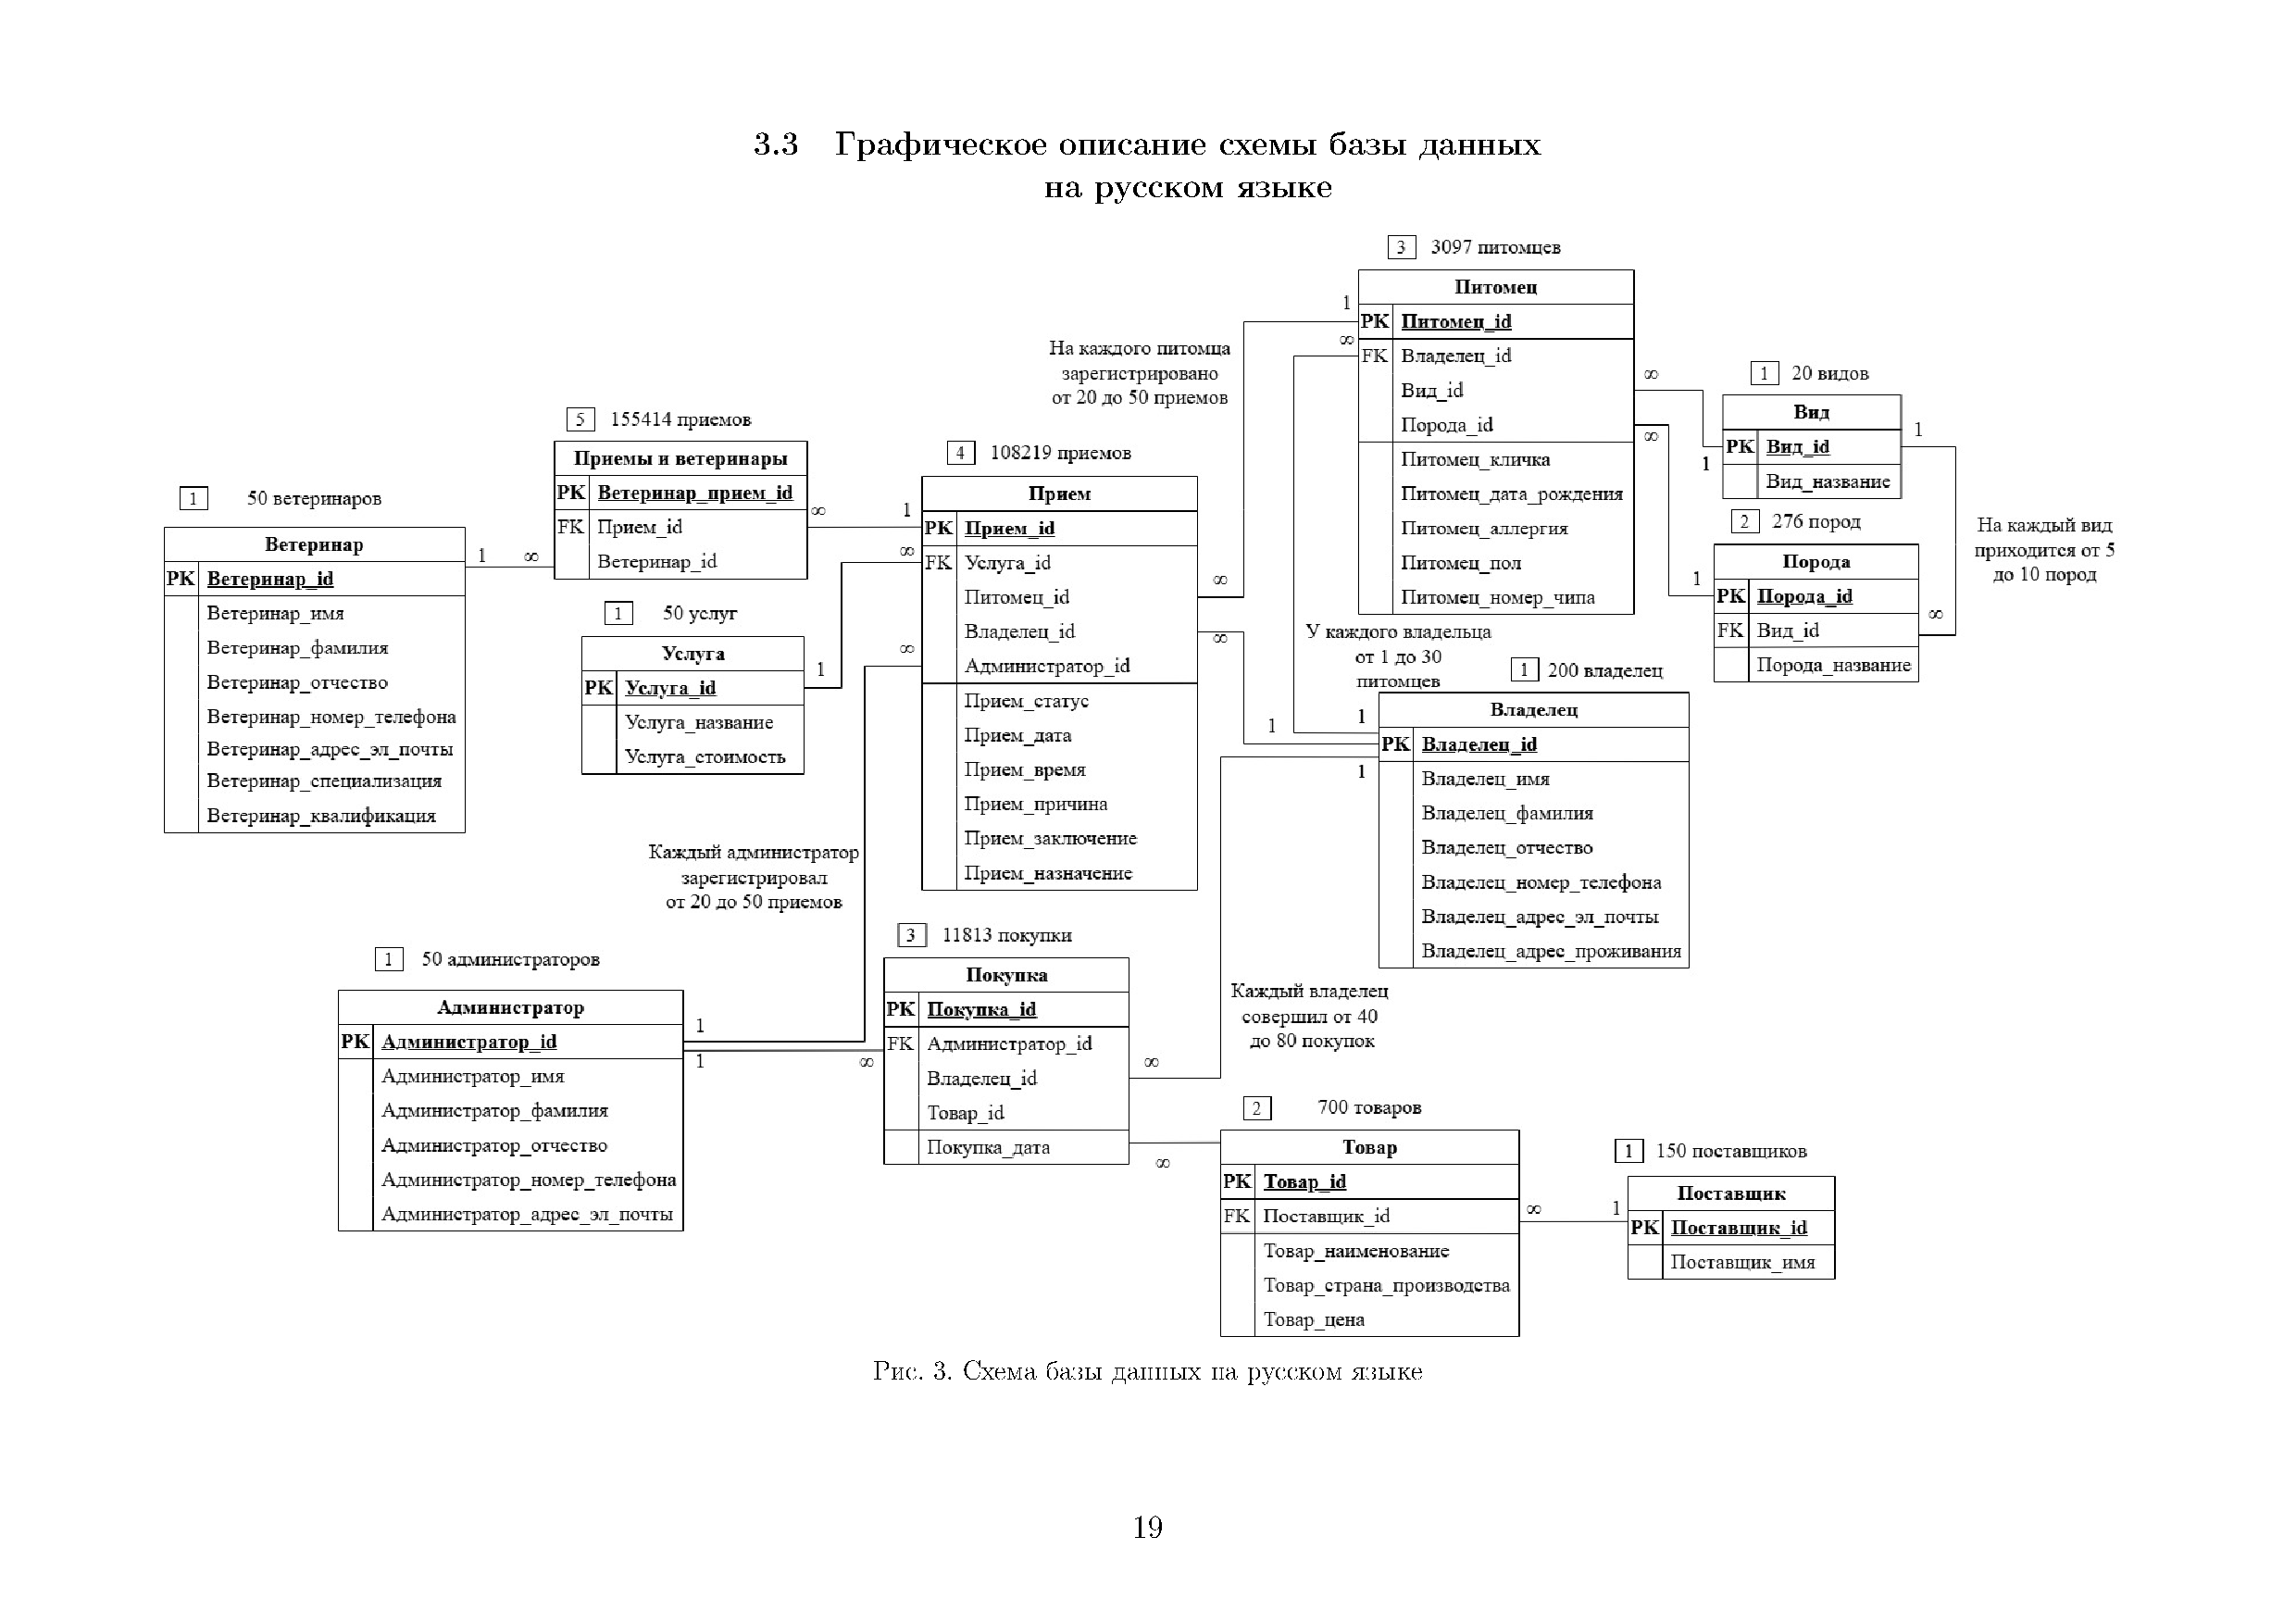
\includepdf[fitpaper]{shemaBD.pdf}
\addcontentsline{toc}{subsection}{3.3 \hspace{0.36cm}Графическое описание схемы базы данных на русском языке} 

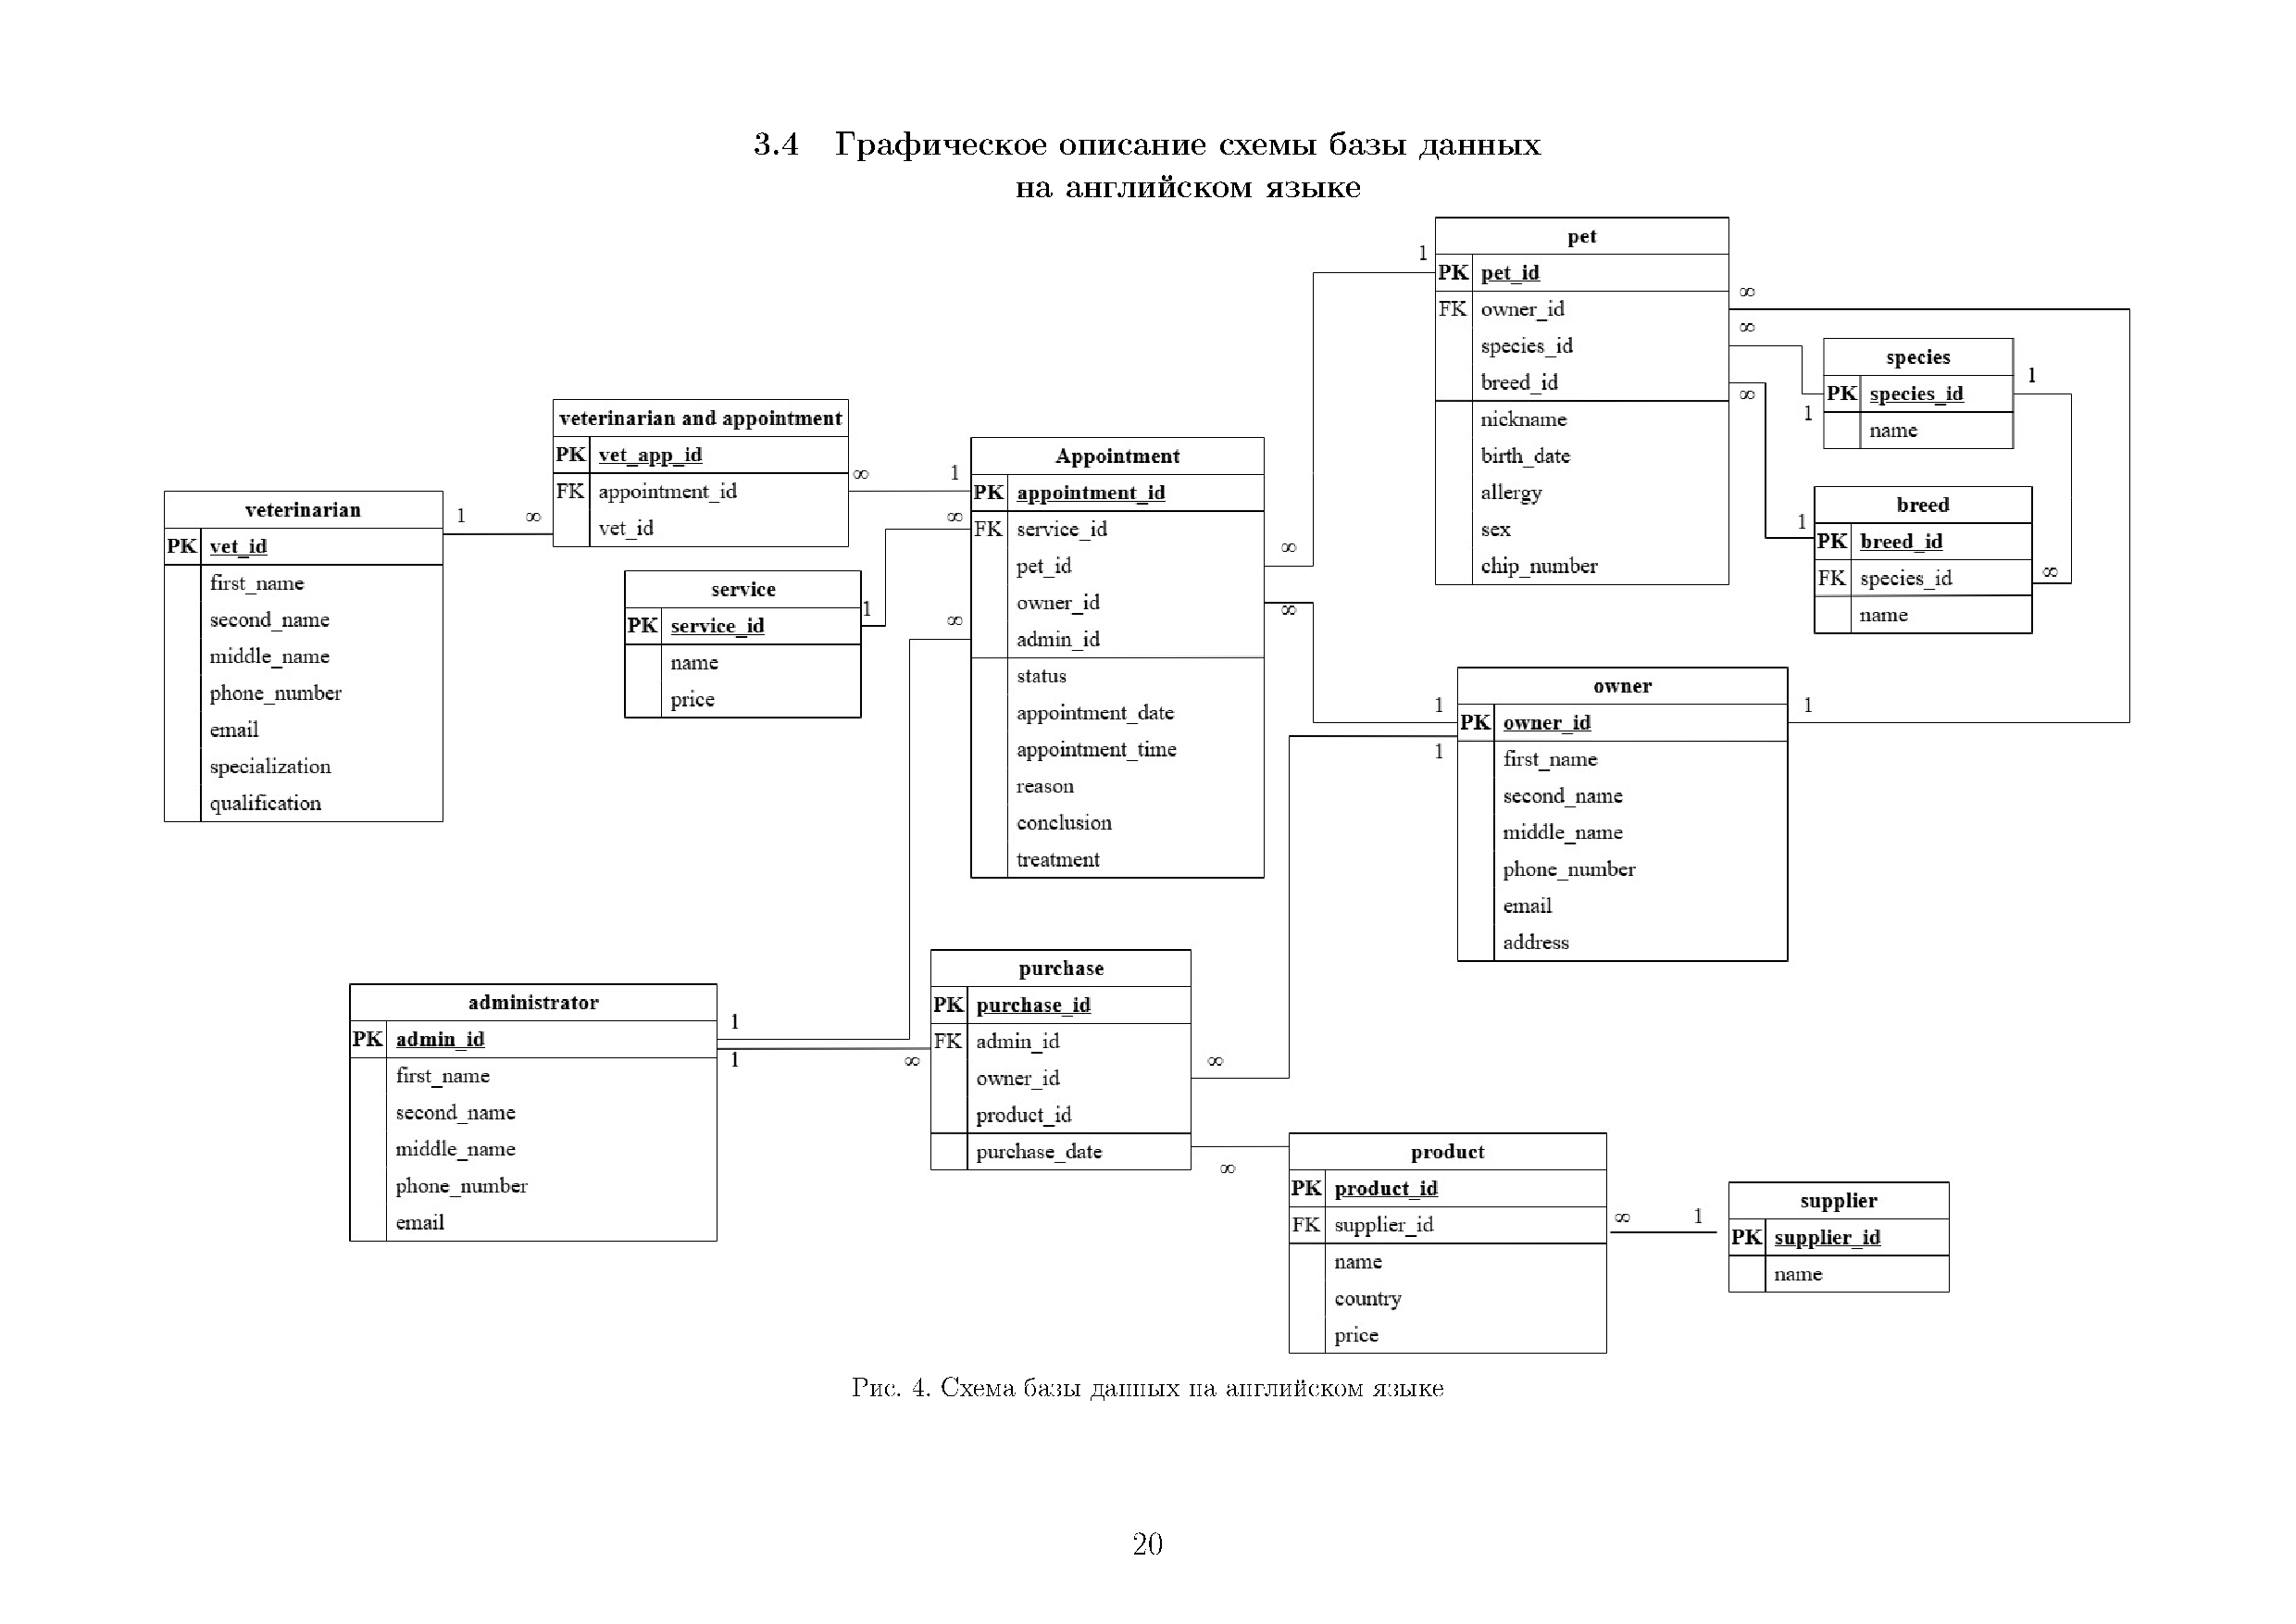
\includepdf[fitpaper]{shemaBDeng.pdf}
\addcontentsline{toc}{subsection}{3.4 \hspace{0.36cm}Графическое описание схемы базы данных на английском языке}

\setcounter{subsection}{4}
\subsection{Создание базы данных и её заполнение}
База данных и содержащиеся в ней таблицы были созданы с помощью SQL-запросов и командной строки MySQL Command Line Client \cite{dbintro}. Исходный код программы создания базы данных приведен в приложении \nameref{section:A}. Графическое представление схемы базы данных на русском и английском языках представлены на рис. 3, 4.

Для заполнения таблиц базы данных была написана программа на языке Python, её исходный текст приведен в приложении \nameref{section:Б}. Был установлен автономный драйвер mysql.connector для взаимодействия с серверами MySQL \cite{pymysql}. Была применена настройка API для подключения к базе данных, в конфигурационном файле были указаны хост, имя пользователя, пароль и имя базы данных. Для выполнения SQL-инструкций использовался курсор -- экземпляр класса MySQLConnection, наследуемый от MySQLCursor. Вставка данных в таблицы производилась с помощью SQL-команд INSERT, перед вставкой данные из таблиц удалялись с помощью команды TRUNCATE. Часть полей таблицы заполнялась с помощью библиотеки Faker -- это пакет Python, который генерирует поддельные данные. 

Всего было выполнено 12 запросов для заполнения 12 таблиц, которые содержат 280039 записей. Распределение записей по таблицам представлено в таблице \ref{tab:записи}.

\begin{table}[H] 
\caption{Количество записей в таблицах}
  \resizebox{\columnwidth}{!}{%
     \begin{tabular}{|c|c|c|}
      \hline
      \cline{1-3}
      \bf №&\bfНазвание таблицы&\bfКоличество записей в таблице\\ 
      \cline{1-3}
      1 & Вид - species & 20 \\ \hline
      2 & Порода - breed & 276 \\ \hline
      3 & Владелец - owners & 200 \\ \hline
      4 & Питомец - pet & 3097 \\ \hline
      5 & Услуга - service & 50 \\ \hline
      6 & Администратор - administrator & 50 \\ \hline
      7 & Прием - appointment & 108219 \\ \hline
      8 & Ветеринар - veterinarian & 50 \\ \hline
      9 & Приемы и ветеринары - veterinarian and appointment & 155414 \\ \hline
      10 & Поставщик - supplier & 150 \\ \hline
      11 & Товар - product & 700 \\ \hline
      12 & Покупка - purchase & 11813 \\ 
      \hline
    \end{tabular}\mbox{} 
  }
  \label{tab:записи}
\end{table}

\newpage
\section{Программирование}
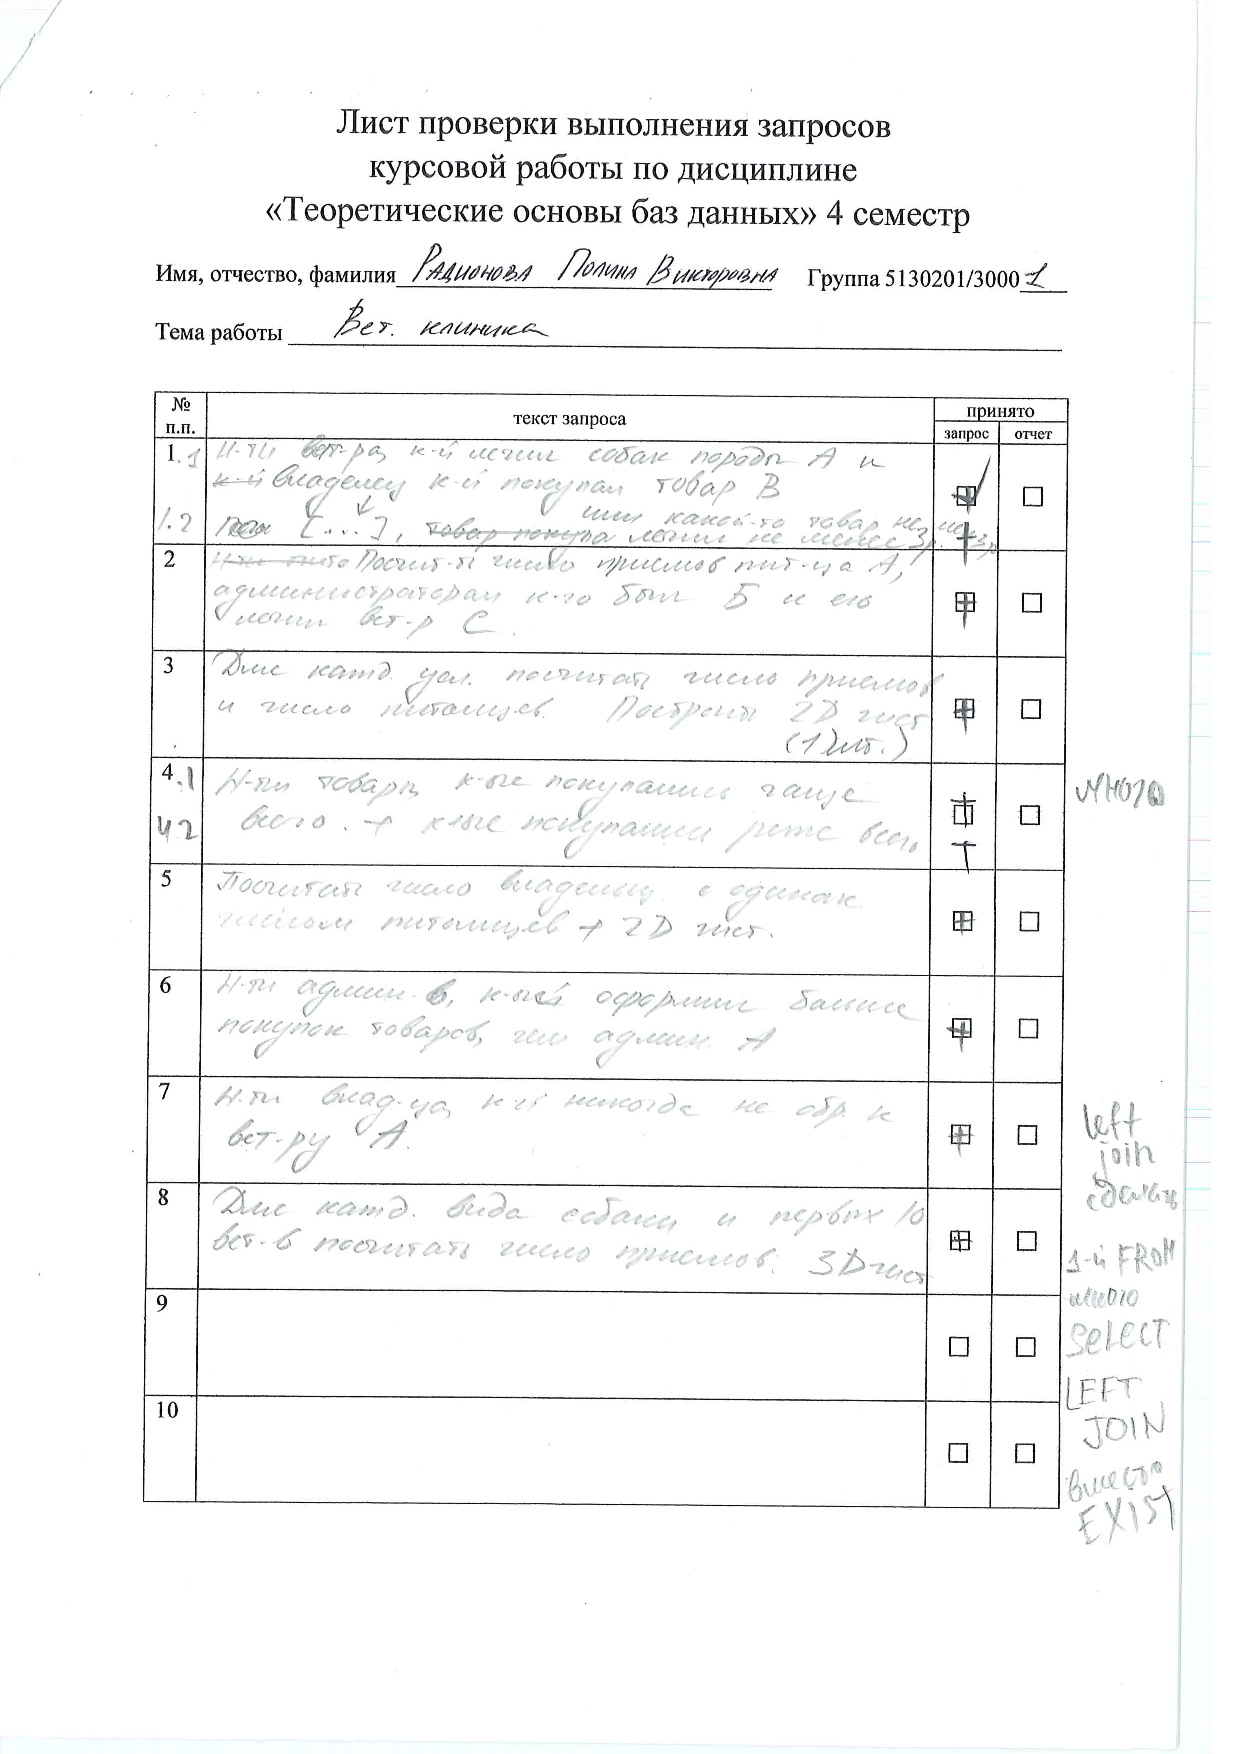
\includepdf{запросы.pdf}
\subsection{Запрос 1.1}
\subsubsection*{Формулировка запроса}
Найти ветеринаров, которые лечили собак породы А, владельцы которых покупали товар B.

\subsubsection*{Реляционная формула запроса}
$$\delta\Bigg(\pi\begin{pmatrix}
    \beta(\text{v.vet\_id}), \\
    \beta(\text{v.first\_name),} \\
    \beta(\text{v.second\_name}), \\
    \beta(\text{v.middle.name})
\end{pmatrix}$$
\vspace{-0.5cm}
$$\sigma(\text{s.name = 'Собака' and b.name = 'Пудель' and prod.name = 'Гигиена}$$
\vspace{-0.9cm}
$$\text{салфетки пасть'})$$
\vspace{-0.5cm}
$$\text{veterinarian} \bowtie (\text{veterinarian.vet\_id = va.vet\_id})\text{veterinarian\_appointment}$$
\vspace{-0.9cm}
$$\text{veterinarian\_appointment}\bowtie(\text{va.appointment\_id = a.appointment\_id)}$$
\vspace{-0.9cm}
$$\text{appointment}$$
\vspace{-0.9cm}
$$\text{appointment}\bowtie(\text{a.pet\_id = p.pet\_id) pet}$$
\vspace{-0.9cm}
$$\text{pet}\bowtie(\text{pet.breed\_id = b.breed\_id) breed}$$
\vspace{-0.9cm}
$$\text{breed}\bowtie(\text{b.species\_id = s.species\_id) species}$$
\vspace{-0.9cm}
$$\text{pet}\bowtie(\text{p.owner\_id = o.owner\_id) owners}$$
\vspace{-0.9cm}
$$\text{owners}\bowtie(\text{o.owner\_id = pur.owner\_id) purchase}$$
\vspace{-0.9cm}
$$\text{purchase}\bowtie(\text{pur.product\_id = prod.product\_id) product}$$

\subsubsection*{Код запроса}
\begin{minted}
[
linenos,tabsize=2,breaklines
]
{sql}
SELECT DISTINCT 
    v.vet_id, 
    v.first_name, 
    v.second_name, 
    v.middle_name
FROM 
    veterinarian v
JOIN veterinarian_appointment va ON v.vet_id = va.vet_id
JOIN appointment a ON va.appointment_id = a.appointment_id
JOIN pet p ON a.pet_id = p.pet_id
JOIN breed b ON p.breed_id = b.breed_id
JOIN species s ON b.species_id = s.species_id
JOIN owners o ON p.owner_id = o.owner_id
JOIN purchase pur ON o.owner_id = pur.owner_id
JOIN product prod ON pur.product_id = prod.product_id
WHERE 
    s.name = 'Собака' 
    AND b.name = 'Пудель' 
    AND prod.name = 'Гигиена салфетки пасть';
\end{minted} 

\setcounter{figure}{4}
\subsubsection*{Результаты запроса}
В результате выполнения запроса было выведено 46 строк. Время выполнения запроса составило 0.047 секунд. Результат запроса представлен на рис. \ref{fig:res1.1}. Табличное и графическое представления последовательности выполнения запроса представлены на рис. \ref{fig:t1.1} и \ref{fig:g1.1} соответственно.

\begin{figure}[h!]
\begin{center}
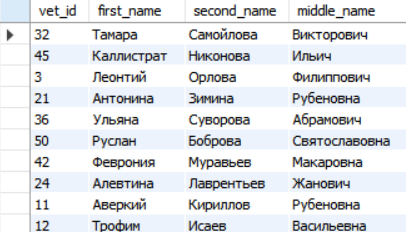
\includegraphics[width=10cm]{resTable_1.1.png}
\captionsetup{justification=centering}
\caption{Результат выполнения запроса 1.1 в виде фрагмента таблицы}
\label{fig:res1.1}
\centering
\end{center}
\end{figure}

\begin{figure}[h!]
\begin{center}
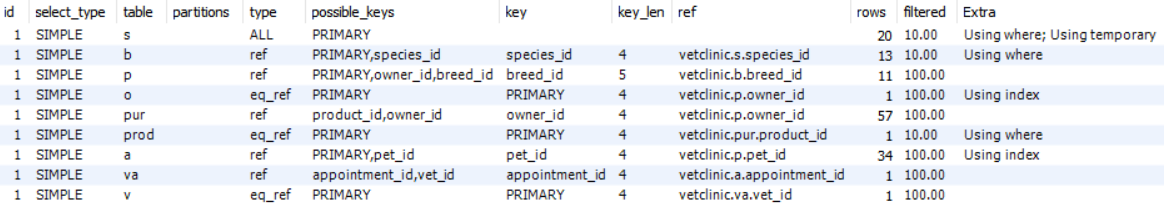
\includegraphics[width=\textwidth]{explainT1.1.png}
\captionsetup{justification=centering}
\caption{Табличное представление последовательности выполнения запроса 1.1}
\label{fig:t1.1}
\centering
\end{center}
\end{figure}

\begin{figure}[h!]
\begin{center}
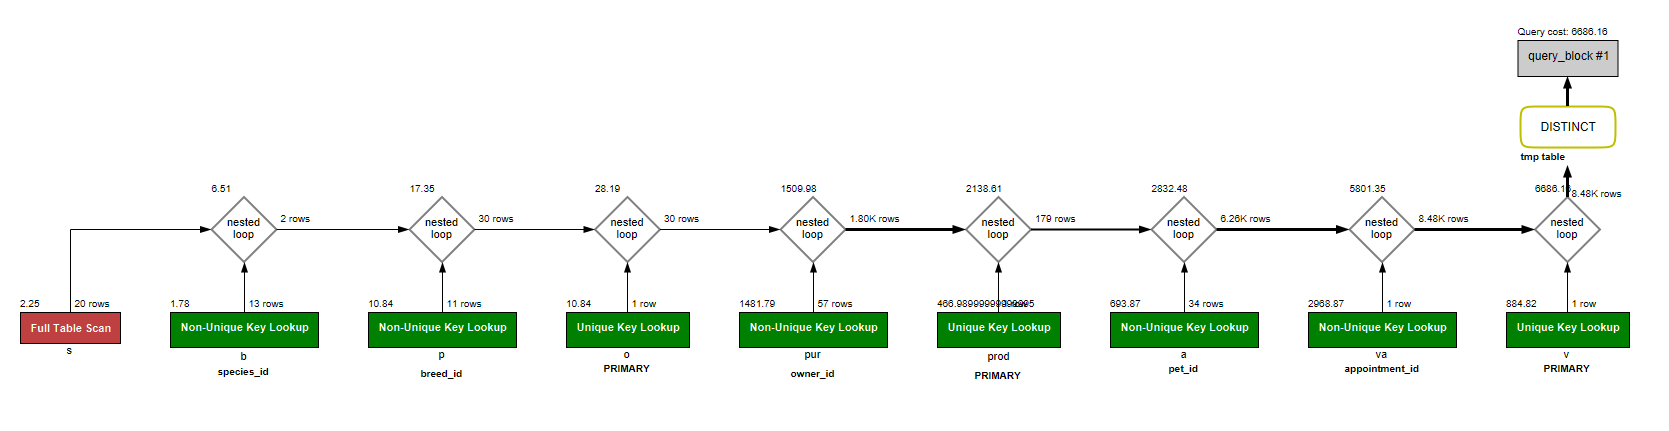
\includegraphics[width=\textwidth]{explainG1.1.png}
\captionsetup{justification=centering}
\caption{Графическое представление последовательности выполнения запроса 1.1}
\label{fig:g1.1}
\centering
\end{center}
\end{figure}

\subsection{Запрос 1.2}
\subsubsection*{Формулировка запроса}
Найти ветеринаров, которые не менее 3-х раз лечили собак породы А, владельцы которых покупали товар B.

\subsubsection*{Код запроса}
\begin{minted}
[
linenos,tabsize=2,breaklines
]
{sql}
SELECT 
    v.vet_id, 
    v.first_name, 
    v.second_name, 
    v.middle_name, 
    COUNT(*) as treatment_count
FROM 
    veterinarian v
JOIN veterinarian_appointment va ON v.vet_id = va.vet_id
JOIN appointment a ON va.appointment_id = a.appointment_id
JOIN pet p ON a.pet_id = p.pet_id
JOIN breed b ON p.breed_id = b.breed_id
JOIN species s ON b.species_id = s.species_id
JOIN owners o ON p.owner_id = o.owner_id
JOIN purchase pur ON o.owner_id = pur.owner_id
JOIN product prod ON pur.product_id = prod.product_id
WHERE 
    s.name = 'Собака' 
    AND b.name = 'Пудель' 
    AND prod.name = 'Гигиена салфетки пасть'
GROUP BY 
    v.vet_id, v.first_name, v.second_name, v.middle_name
HAVING COUNT(*) >= 3;
\end{minted} 

\subsubsection*{Текстовое объяснение запроса}
Запрос с помощью JOIN выполняет соединение 10 таблиц по следующим ключам:
\begin{itemize}
    \item veterinarian.vet\_id $\to$ veterinarian\_appointment.vet\_id;
    \item veterinarian\_appointment.appointment\_id $\to$ appointment.appointme- nt\_id;
    \item appointment.pet\_id $\to$ pet.pet\_id;
    \item pet.breed\_id $\to$ breed.breed\_id;
    \item breed.species\_id $\to$ species.species\_id;
    \item pet.owner\_id $\to$ owners.owner\_id;
    \item owners.owner\_id $\to$ purchase.owner\_id;
    \item purchase.product\_id $\to$ product.product\_id.
\end{itemize}
Далее с помощью WHERE выбираются записи, соответствующие указанным значениям для species.name, breed.name и product.name. Полученные строки группируются по ветеринарам с помощью GROUP BY veterinarian.vet\_id, veterinarian.first\_name, veterinarian.second\_name, 
vet-erinarian.middle\_name, чтобы избежать дублирования строк. В конце c помощью фильтрации HAVING COUNT(*) >= 3 остаются только подходящие ветеринары. 

\subsubsection*{Результаты запроса}
В результате выполнения запроса была выведена 21 строка. Время выполнения запроса составило 0.047 секунд. Результат запроса представлен на рис. \ref{fig:res1.2}. Табличное и графическое представления последовательности выполнения запроса представлены на рис. \ref{fig:t1.2} и \ref{fig:g1.2} соответственно.

\begin{figure}[h!]
\begin{center}
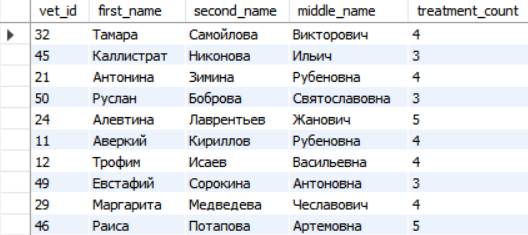
\includegraphics[width=10cm]{resTable_1.2.png}
\captionsetup{justification=centering}
\caption{Результат выполнения запроса 1.2 в виде фрагмента таблицы}
\label{fig:res1.2}
\centering
\end{center}
\end{figure}

\begin{figure}[h!]
\begin{center}
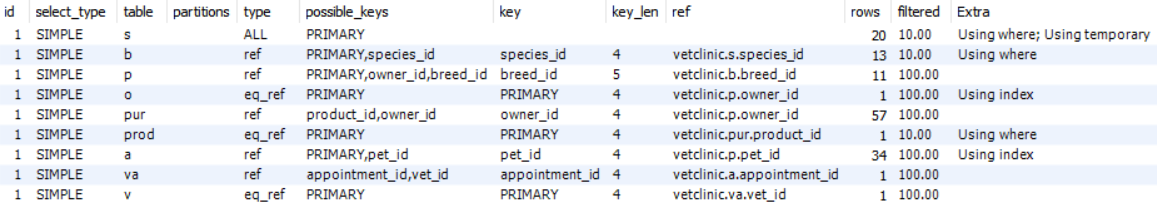
\includegraphics[width=\textwidth]{explainT1.2.png}
\captionsetup{justification=centering}
\caption{Табличное представление последовательности выполнения запроса 1.2}
\label{fig:t1.2}
\centering
\end{center}
\end{figure}

\begin{figure}[h!]
\begin{center}
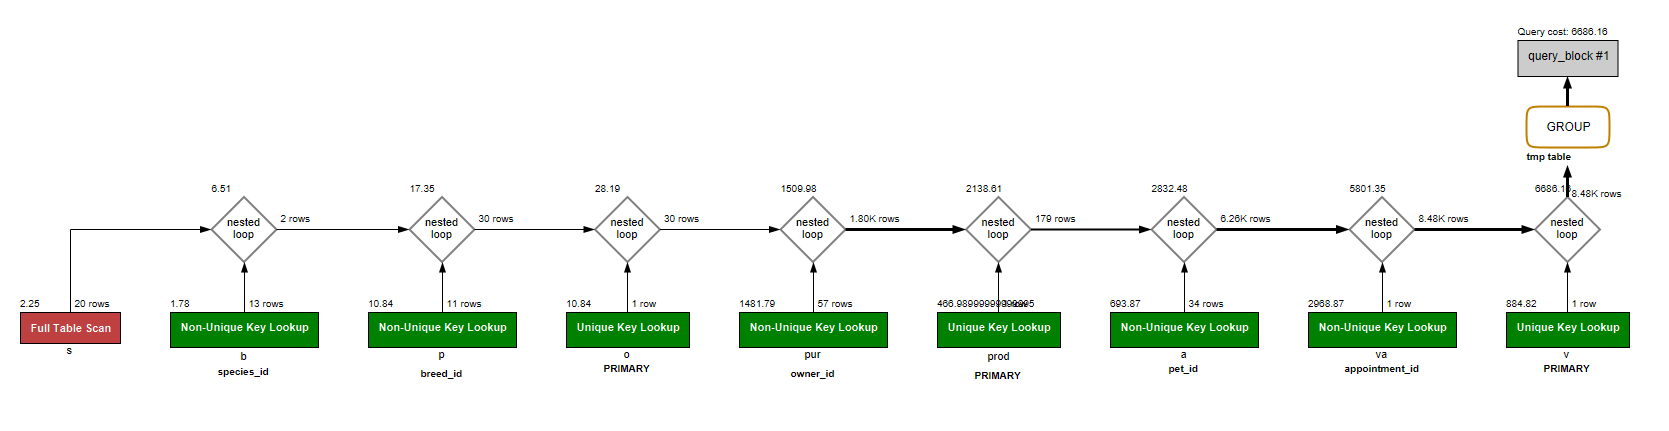
\includegraphics[width=\textwidth]{explainG1.2.png}
\captionsetup{justification=centering}
\caption{Графическое представление последовательности выполнения запроса 1.2}
\label{fig:g1.2}
\centering
\end{center}
\end{figure}

\subsection{Запрос 2}
\subsubsection*{Формулировка запроса}
Посчитать число приемов питомца A, администратором которого был администратор B и ветеринаром которого был ветеринар C.

\subsubsection*{Реляционная формула запроса}
$$\pi(\beta(\text{COUNT(*) AS appointment\_count}))$$
$$\sigma(\text{pet.pet\_id=1 and adm.second\_name = 'Рожкова' and v.second\_name=}$$
\vspace{-0.9cm}
$$=\text{'Рогова'})$$
$$\text{appointment}\bowtie(\text{a.pet\_id = p.pet\_id})\text{pet}$$
\vspace{-0.9cm}
$$\text{administrator}\bowtie(\text{a.admin\_id = adm.admin\_id})\text{appointment}$$
\vspace{-0.9cm}
$$\text{veterinarian\_appointment}\bowtie(\text{a.appointment\_id = va.appointment\_id})$$
\vspace{-0.9cm}
$$\text{appointment}$$
\vspace{-0.9cm}
$$\text{veterinarian}\bowtie(\text{va.vet\_id = v.vet\_id})\text{veterinarian\_appointment}$$

\subsubsection*{Код запроса}
\begin{minted}
[
linenos,tabsize=2,breaklines
]
{sql}
SELECT 
    COUNT(*) AS appointment_count
FROM 
    appointment a
JOIN pet p ON a.pet_id = p.pet_id
JOIN administrator adm ON a.admin_id = adm.admin_id
JOIN veterinarian_appointment va ON a.appointment_id = va.appointment_id
JOIN veterinarian v ON va.vet_id = v.vet_id
WHERE 
    p.pet_id = 1
    AND adm.second_name = 'Рожкова' 
    AND v.second_name = 'Рогова';
\end{minted} 

\subsubsection*{Текстовое объяснение запроса}
С помощью JOIN запрос соединяет таблицы appointment, pet, administrator, veterinarian\_appointment и veterinarian по следующим ключам:
\begin{itemize}
    \item $\text{appointment.pet\_id} \to \text{pet.pet\_id}$;
    \item $\text{appointment.admin\_id} \to \text{administrator.admin\_id}$;
    \item $\text{appointment.appointment\_id} \to \text{veterinarian\_appointment.appointment\_id}$;
    \item $\text{veterinarian\_appointment.vet\_id} \to \text{veterinarian.vet\_id}$.
\end{itemize}
Далее с помощью WHERE выбираются только записи, соответствующие указанным значениям для pet.pet\_id, administrator.second\_name и veterinarian.second\_name. С использованием COUNT(*) подсчитывается общее количество приемов appointment\_count, удовлетворяющих заданным условиям. 

\subsubsection*{Результаты запроса}
В результате выполнения запроса была выведена 1 строка. Время выполнения запроса составило 0.016 секунд. Результат запроса представлен на рис. \ref{fig:res2}. Табличное и графическое представления последовательности выполнения запроса представлены на рис. \ref{fig:t2} и \ref{fig:g2} соответственно.

\begin{figure}[h!]
\begin{center}

\includegraphics[width=6cm]{resTable_2.png}
\captionsetup{justification=centering}
\caption{Результат выполнения запроса 2 в виде таблицы}
\label{fig:res2}
\centering
\end{center}
\end{figure}

\begin{figure}[h!]
\begin{center}
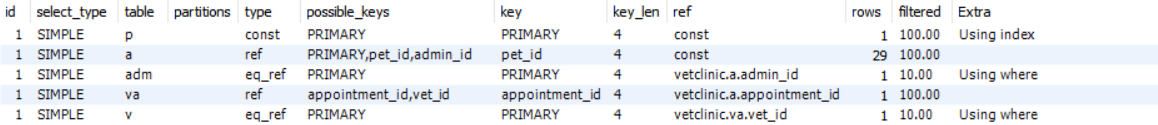
\includegraphics[width=\textwidth]{explainT2.png}
\captionsetup{justification=centering}
\caption{Табличное представление последовательности выполнения запроса 2}
\label{fig:t2}
\centering
\end{center}
\end{figure}

\begin{figure}[h!]
\begin{center}
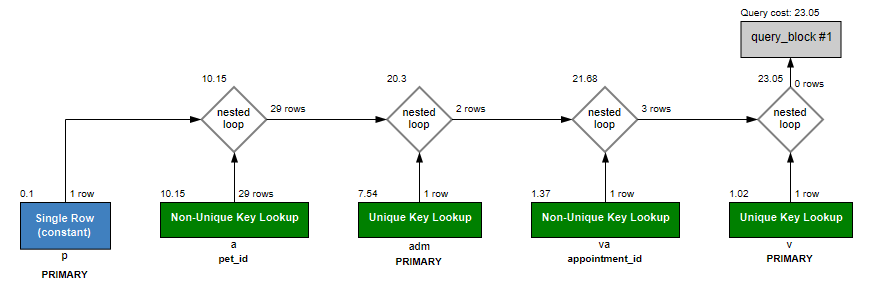
\includegraphics[width=14cm]{explainG2.png}
\captionsetup{justification=centering}
\caption{Графическое представление последовательности выполнения запроса 2}
\label{fig:g2}
\centering
\end{center}
\end{figure}

\subsection{Запрос 3}
\subsubsection*{Формулировка запроса}
Для каждой услуги посчитать число приемов и число питомцев.

\subsubsection*{Реляционная формула запроса}
$$\pi\begin{pmatrix}
    \beta({\text{s.service\_id}),\\
    \beta(\text{s.name AS service\_name}),\\
    \beta(\text{COUNT(a.appointment\_id) AS total\_appointments}),\\
    \beta(\text{COUNT(DISTINCT a.pet\_id) AS unique\_pets})
\end{pmatrix}$$
$$\text{service}\bowtie\text{(service.service\_id=appointment.service\_id) appointment}$$
$$\gamma(\text{service.service\_id, service.name})$$

\subsubsection*{Код запроса}
\begin{minted}
[
linenos,tabsize=2,breaklines
]
{sql}
SELECT 
    s.service_id,  
    s.name AS service_name,
    COUNT(a.appointment_id) AS total_appointments,
    COUNT(DISTINCT a.pet_id) AS unique_pets
FROM 
    service s
LEFT JOIN 
    appointment a ON s.service_id = a.service_id
GROUP BY 
    s.service_id, s.name  
ORDER BY 
    s.service_id;
\end{minted} 

\subsubsection*{Результаты запроса}
В результате выполнения запроса было выведено 50 строк. Время выполнения запроса составило 0.469 секунд. Результат запроса представлен на рис. \ref{fig:res3}. Табличное и графическое представления последовательности выполнения запроса представлены на рис. \ref{fig:t3} и \ref{fig:g3} соответственно.

\begin{figure}[h!]
\begin{center}
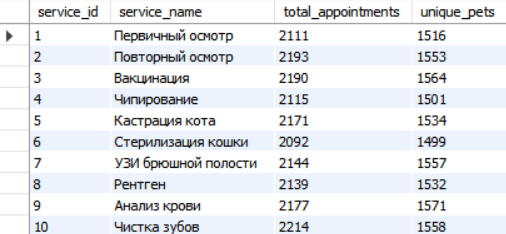
\includegraphics[width=10cm]{resTable_3.png}
\captionsetup{justification=centering}
\caption{Результат выполнения запроса 3 в виде фрагмента таблицы}
\label{fig:res3}
\centering
\end{center}
\end{figure}

\begin{figure}[h!]
\begin{center}

\includegraphics[width=\textwidth]{explainT3.png}
\captionsetup{justification=centering}
\caption{Табличное представление последовательности выполнения запроса 3}
\label{fig:t3}
\centering
\end{center}
\end{figure}

\begin{figure}[h!]
\begin{center}
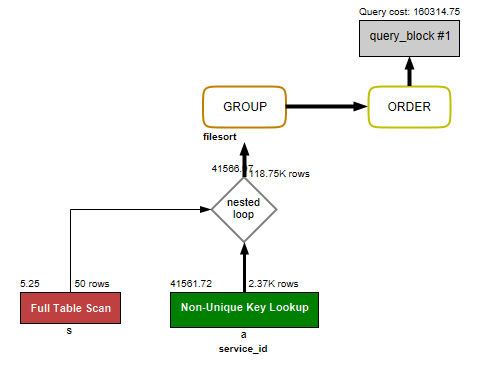
\includegraphics[width=10cm]{explainG3.png}
\captionsetup{justification=centering}
\caption{Графическое представление последовательности выполнения запроса 3}
\label{fig:g3}
\centering
\end{center}
\end{figure}

\subsubsection*{Гистограмма запроса}
На рис. \ref{fig:gist3} представлена 2D-гистограмма, демонстрирующая распределение приемов и уникальных питомцев по всем имеющимся в таблице услугам.
\begin{figure}[h!]
\begin{center}
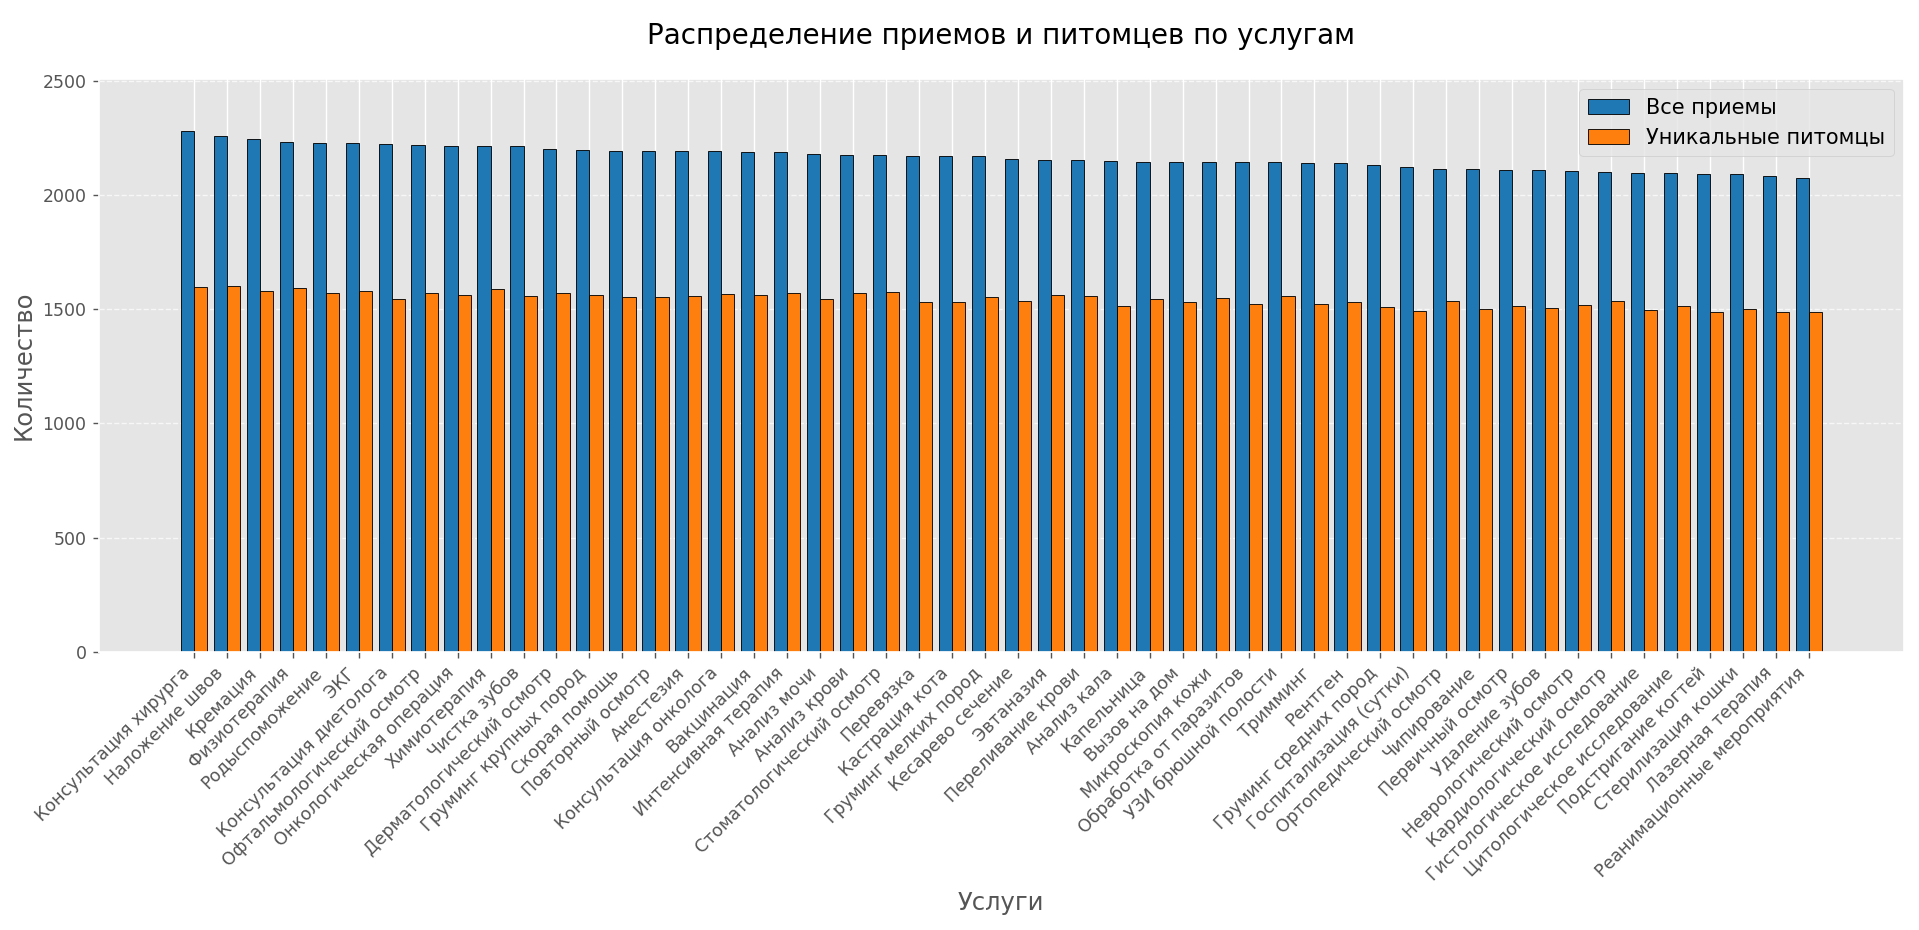
\includegraphics[width=\textwidth]{gist3.png}
\captionsetup{justification=centering}
\caption{Гистограмма запроса 3}
\label{fig:gist3}
\centering
\end{center}
\end{figure}

\subsection{Запрос 4.1}
\subsubsection*{Формулировка запроса}
Найти товары, которые покупались чаще всего.

\subsubsection*{Реляционная формула запроса}

$$\pi\begin{pmatrix}
    \beta({\text{product.name AS product\_name}),\\
    \beta(\text{COUNT(purchase.product\_id) AS total\_purchase})
\end{pmatrix}$$
$$\text{purchase}\bowtie\text{(purchase.product\_id=product.product\_id) product}$$
$$\gamma(\text{service.service\_id, service.name})$$

\subsubsection*{Код запроса}
\begin{minted}
[
linenos,tabsize=2,breaklines
]
{sql}
SELECT 
    product.name AS product_name,
    COUNT(purchase.product_id) AS total_purchases
FROM
    purchase
        JOIN
    product ON purchase.product_id = product.product_id
GROUP BY purchase.product_id
HAVING COUNT(purchase.product_id) = (SELECT 
        MAX(purchase_count)
    FROM
        (SELECT 
            COUNT(product_id) AS purchase_count
        FROM
            purchase
        GROUP BY product_id) AS counts);
\end{minted} 

\subsubsection*{Результаты запроса}
В результате выполнения запроса было выведено 2 строки. Время выполнения запроса составило 0.053 секунды. Результат запроса представлен на рис. \ref{fig:res4.1}. Табличное и графическое представления последовательности выполнения запроса представлены на рис. \ref{fig:t4.1} и \ref{fig:g4.1} соответственно.

\begin{figure}[h!]
\begin{center}

\includegraphics[width=10cm]{resTable_4.1.png}
\captionsetup{justification=centering}
\caption{Результат выполнения запроса 4.1 в виде таблицы}
\label{fig:res4.1}
\centering
\end{center}
\end{figure}

\begin{figure}[h!]
\begin{center}
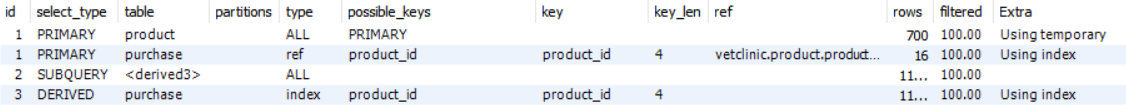
\includegraphics[width=\textwidth]{explainT4.1.png}
\captionsetup{justification=centering}
\caption{Табличное представление последовательности выполнения запроса 4.1}
\label{fig:t4.1}
\centering
\end{center}
\end{figure}

\begin{figure}[h!]
\begin{center}
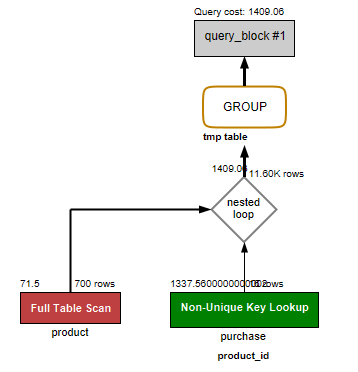
\includegraphics[width=12cm]{explainG4.1.png}
\captionsetup{justification=centering}
\caption{Графическое представление последовательности выполнения запроса 4.1}
\label{fig:g4.1}
\centering
\end{center}
\end{figure}

\subsection{Запрос 4.2}
\subsubsection*{Формулировка запроса}
Найти товары, которые покупались реже всего.

\subsubsection*{Код запроса}
\begin{minted}
[
linenos,tabsize=2,breaklines
]
{sql}
SELECT 
    product.name AS product_name,
    COUNT(purchase.product_id) AS total_purchases
FROM
    purchase
        JOIN
    product ON purchase.product_id = product.product_id
GROUP BY purchase.product_id
HAVING COUNT(purchase.product_id) = (SELECT 
        MIN(purchase_count)
    FROM
        (SELECT 
            COUNT(product_id) AS purchase_count
        FROM
            purchase
        GROUP BY product_id) AS counts);
\end{minted} 

\subsubsection*{Результаты запроса}
В результате выполнения запроса была выведена 1 строка. Время выполнения запроса составило 0.053 секунды. Результат запроса представлен на рис. \ref{fig:res4.2}. Табличное и графическое представления последовательности выполнения запроса представлены на рис. \ref{fig:t4.2} и \ref{fig:g4.2} соответственно.

\begin{figure}[h!]
\begin{center}

\includegraphics[width=10cm]{resTable_4.2.png}
\captionsetup{justification=centering}
\caption{Результат выполнения запроса 4.2 в виде таблицы}
\label{fig:res4.2}
\centering
\end{center}
\end{figure}

\begin{figure}[h!]
\begin{center}
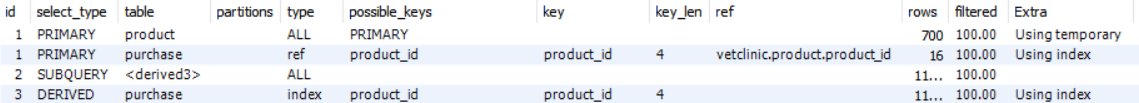
\includegraphics[width=\textwidth]{explainT4.2.png}
\captionsetup{justification=centering}
\caption{Табличное представление последовательности выполнения запроса 4.2}
\label{fig:t4.2}
\centering
\end{center}
\end{figure}

\begin{figure}[h!]
\begin{center}
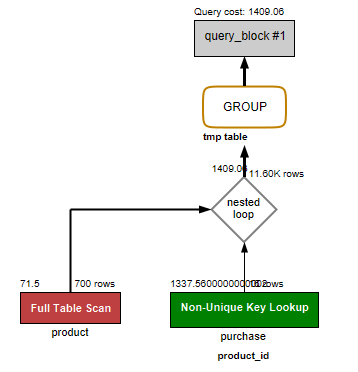
\includegraphics[width=12cm]{explainG4.2.png}
\captionsetup{justification=centering}
\caption{Графическое представление последовательности выполнения запроса 4.2}
\label{fig:g4.2}
\centering
\end{center}
\end{figure}

\subsection{Запрос 5}
\subsubsection*{Формулировка запроса}
Посчитать число владельцев с одинаковым количеством питомцев.

\subsubsection*{Код запроса}
\begin{minted}
[
linenos,tabsize=2,breaklines
]
{sql}
SELECT 
    pet_counts.pet_count,
    COUNT(pet_counts.owner_id) AS owner_count
FROM (
    SELECT 
        o.owner_id,
        COUNT(p.pet_id) AS pet_count
    FROM 
        owners o
    LEFT JOIN 
        pet p ON o.owner_id = p.owner_id
    GROUP BY 
        o.owner_id
) AS pet_counts
GROUP BY 
    pet_counts.pet_count
ORDER BY 
    pet_counts.pet_count;
\end{minted} 

\subsubsection*{Текстовое объяснение запроса}
В запросе используется подзапрос pet\_counts, который соединяет таблицы owners и pet через LEFT JOIN по полю owner\_id, группирует результат соединения по owner\_id и для каждого владельца считает количество его питомцев COUNT(p.pet\_id).

Далее основной запрос обрабатывает результаты подзапроса: он группирует данные по количеству питомцев, для каждой группы подсчитывает количество владельцев. В конце происходит сортировка результатов по возрастанию количества питомцев.

\subsubsection*{Результаты запроса}
В результате выполнения запроса было выведено 30 строк. Время выполнения запроса составило 0.043 секунды. Результат запроса представлен на рис. \ref{fig:res5}. Табличное и графическое представления последовательности выполнения запроса представлены на рис. \ref{fig:t5} и \ref{fig:g5} соответственно.

\begin{figure}[h!]
\begin{center}
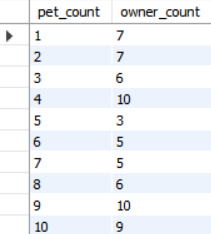
\includegraphics[width=5cm]{resTable_5.png}
\captionsetup{justification=centering}
\caption{Результат выполнения запроса 5 в виде фрагмента таблицы}
\label{fig:res5}
\centering
\end{center}
\end{figure}

\begin{figure}[h!]
\begin{center}

\includegraphics[width=\textwidth]{explainT5.png}
\captionsetup{justification=centering}
\caption{Табличное представление последовательности выполнения запроса 5}
\label{fig:t5}
\centering
\end{center}
\end{figure}

\begin{figure}[h!]
\begin{center}
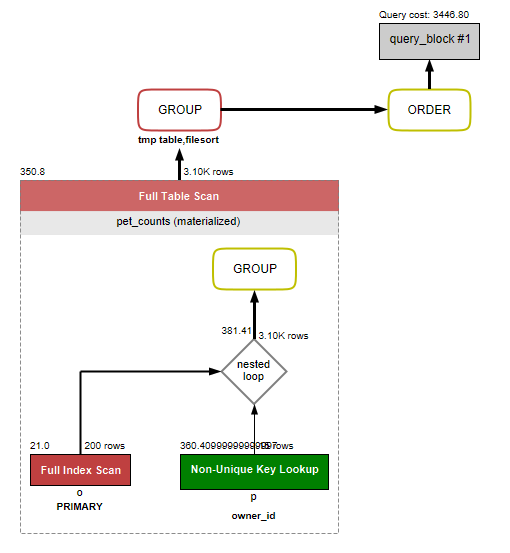
\includegraphics[width=10.3cm]{explainG5.png}
\captionsetup{justification=centering}
\caption{Графическое представление последовательности выполнения запроса 5}
\label{fig:g5}
\centering
\end{center}
\end{figure}

\subsubsection*{Гистограмма запроса}
На рис. \ref{fig:gist5} представлена 2D-гистограмма, демонстрирующая распределение владельцев по количеству питомцев.
\begin{figure}[h!]
\begin{center}
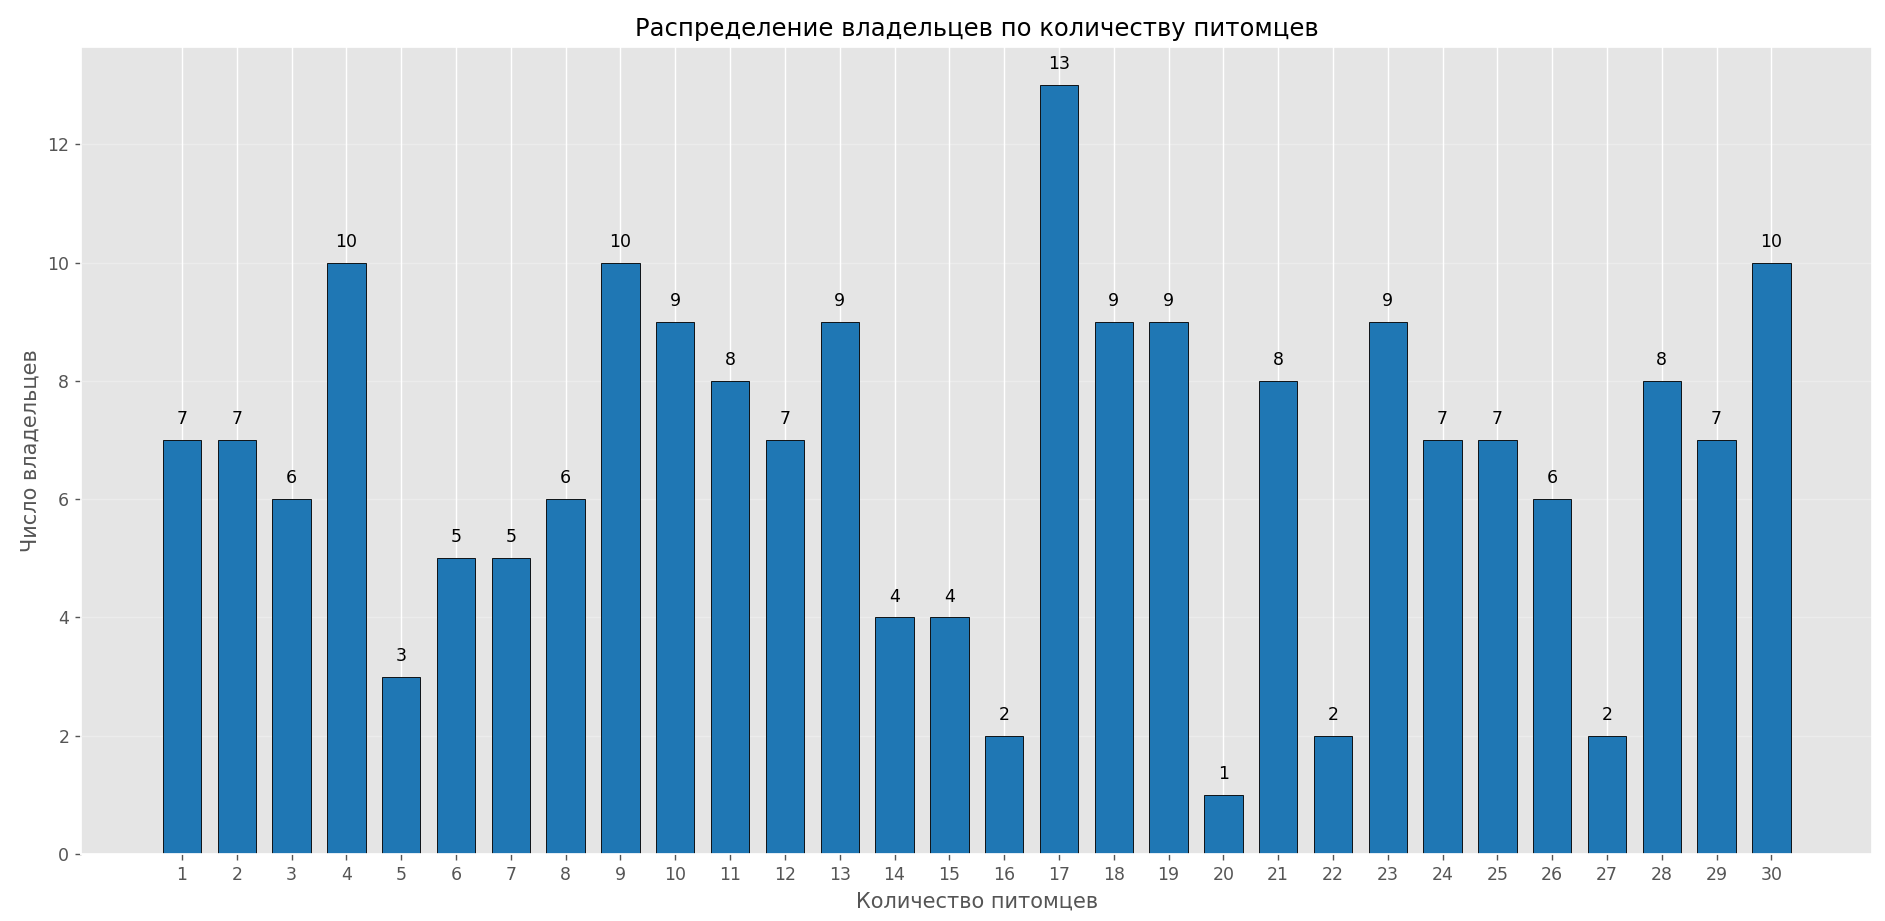
\includegraphics[width=\textwidth]{gist5.png}
\captionsetup{justification=centering}
\caption{Гистограмма запроса 5}
\label{fig:gist5}
\centering
\end{center}
\end{figure}

\subsection{Запрос 6}
\subsubsection*{Формулировка запроса}
Найти администраторов, которые оформили больше покупок, чем администратор A.

\subsubsection*{Код запроса}
\begin{minted}
[
linenos,tabsize=2,breaklines
]
{sql}
SELECT 
    a.admin_id,
    a.first_name,
    a.second_name,
    COUNT(p.purchase_id) AS purchase_count
FROM 
    administrator a
LEFT JOIN 
    purchase p ON a.admin_id = p.admin_id
GROUP BY 
    a.admin_id, a.first_name, a.second_name
HAVING 
    COUNT(p.purchase_id) > (
        SELECT COUNT(p2.purchase_id)
        FROM administrator a2
        LEFT JOIN purchase p2 ON a2.admin_id = p2.admin_id
        WHERE a2.admin_id = 1
        GROUP BY a2.admin_id
    )
ORDER BY 
    purchase_count DESC;
\end{minted} 

\subsubsection*{Результаты запроса}
В результате выполнения запроса было выведено 7 строк. Время выполнения запроса составило 0.078 секунд. Результат запроса представлен на рис. \ref{fig:res6}. Табличное и графическое представления последовательности выполнения запроса представлены на рис. \ref{fig:t6} и \ref{fig:g6} соответственно.

\begin{figure}[h!]
\begin{center}
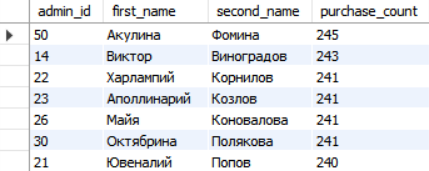
\includegraphics[width=10cm]{resTable_6.png}
\captionsetup{justification=centering}
\caption{Результат выполнения запроса 6 в виде таблицы}
\label{fig:res6}
\centering
\end{center}
\end{figure}

\begin{figure}[h!]
\begin{center}
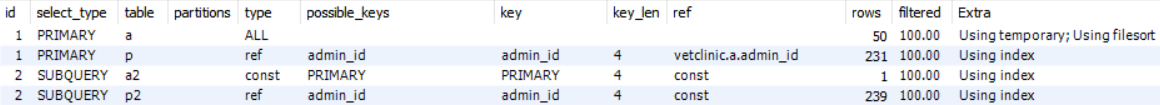
\includegraphics[width=\textwidth]{explainT6.png}
\captionsetup{justification=centering}
\caption{Табличное представление последовательности выполнения запроса 6}
\label{fig:t6}
\centering
\end{center}
\end{figure}

\begin{figure}[h!]
\begin{center}
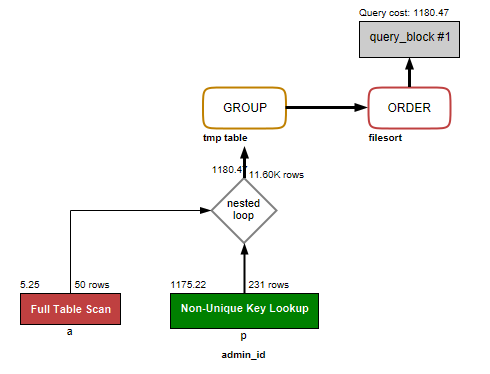
\includegraphics[width=12cm]{explainG6.png}
\captionsetup{justification=centering}
\caption{Графическое представление последовательности выполнения запроса 6}
\label{fig:g6}
\centering
\end{center}
\end{figure}

\subsection{Запрос 7}
\subsubsection*{Формулировка запроса}
Найти владельцев, которые никогда не обращались к ветеринару A.

\subsubsection*{Код запроса}
\begin{minted}
[
linenos,tabsize=2,breaklines
]
{sql}
SELECT 
    o.owner_id,
    o.first_name,
    o.second_name
FROM 
    owners o
WHERE 
    o.owner_id NOT IN (
        SELECT DISTINCT a.owner_id
        FROM appointment a
        JOIN veterinarian_appointment va ON a.appointment_id = va.appointment_id
        WHERE va.vet_id = 10  
    );
\end{minted} 

\subsubsection*{Результаты запроса}
В результате выполнения запроса было выведено 4 строки. Время выполнения запроса составило 0.122 секунды. Результат запроса представлен на рис. \ref{fig:res7}. Табличное и графическое представления последовательности выполнения запроса представлены на рис. \ref{fig:t7} и \ref{fig:g7} соответственно.

\begin{figure}[h!]
\begin{center}
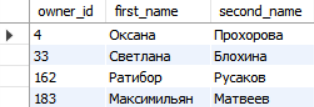
\includegraphics[width=10cm]{resTable_7.png}
\captionsetup{justification=centering}
\caption{Результат выполнения запроса 7 в виде таблицы}
\label{fig:res7}
\centering
\end{center}
\end{figure}

\begin{figure}[h!]
\begin{center}
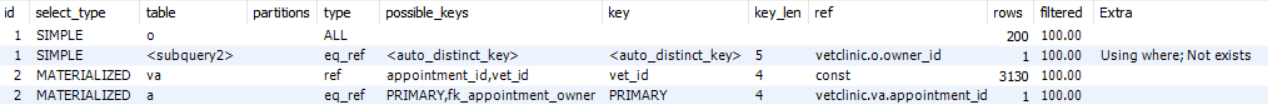
\includegraphics[width=\textwidth]{explainT7.png}
\captionsetup{justification=centering}
\caption{Табличное представление последовательности выполнения запроса 7}
\label{fig:t7}
\centering
\end{center}
\end{figure}

\begin{figure}[h!]
\begin{center}
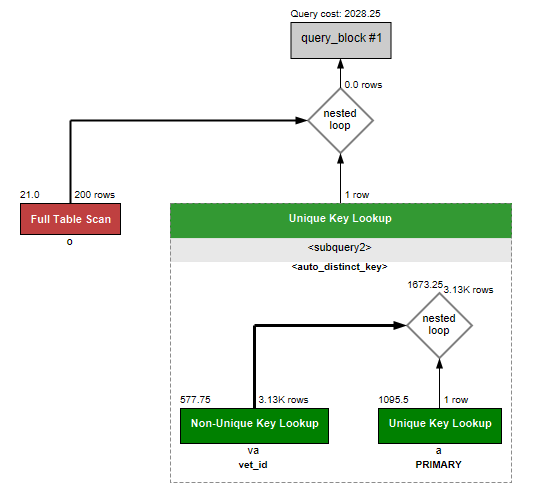
\includegraphics[width=9cm]{explainG7.png}
\captionsetup{justification=centering}
\caption{Графическое представление последовательности выполнения запроса 7}
\label{fig:g7}
\centering
\end{center}
\end{figure}

\subsection{Запрос 8}
\subsubsection*{Формулировка запроса}
Для каждой породы собак и первых 10 ветеринаров посчитать число приемов.

\subsubsection*{Код запроса}
\begin{minted}
[
linenos,tabsize=2,breaklines
]
{sql}
SELECT 
    b.name AS breed_name,
    v.vet_id,
    v.first_name,
    v.second_name,
    COUNT(va.vet_app_id) AS appointment_count
FROM
    (SELECT 
        *
    FROM
        veterinarian
    ORDER BY vet_id
    LIMIT 10) AS v
        CROSS JOIN
    (SELECT 
        b.*
    FROM
        breed b
    JOIN species s ON b.species_id = s.species_id
    WHERE
        s.name = 'Собака') AS b
        LEFT JOIN pet p ON p.breed_id = b.breed_id
        LEFT JOIN appointment a ON a.pet_id = p.pet_id
        LEFT JOIN veterinarian_appointment va ON va.appointment_id = a.appointment_id
        AND va.vet_id = v.vet_id
GROUP BY b.name , v.vet_id , v.first_name , v.second_name
ORDER BY b.name , v.vet_id;
\end{minted} 

\subsubsection*{Результаты запроса}
В результате выполнения запроса было выведено 150 строк. Время выполнения запроса составило 0.312 секунд. Результат запроса представлен на рис. \ref{fig:res8}. 

\begin{figure}[h!]
\begin{center}
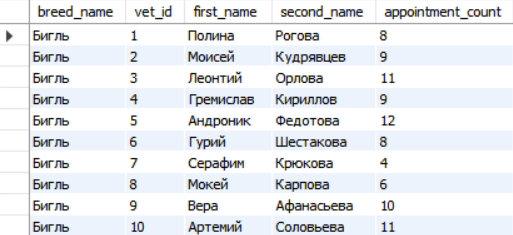
\includegraphics[width=9cm]{resTable_8.png}
\captionsetup{justification=centering}
\caption{Результат выполнения запроса 8 в виде фрагмента таблицы}
\label{fig:res8}
\centering
\end{center}
\end{figure}

Табличное и графическое представления последовательности выполнения запроса представлены на рис. \ref{fig:t8} и \ref{fig:g8} соответственно.

\begin{figure}[h!]
\begin{center}
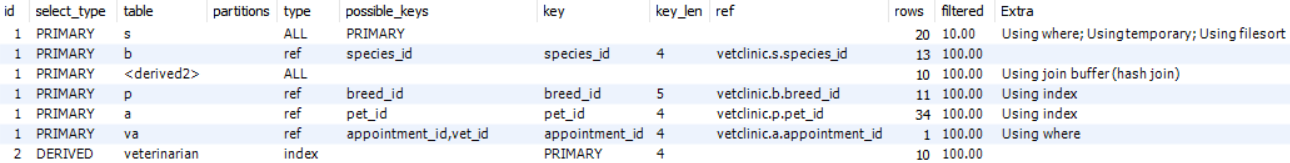
\includegraphics[width=\textwidth]{explainT8.png}
\captionsetup{justification=centering}
\caption{Табличное представление последовательности выполнения запроса 8}
\label{fig:t8}
\centering
\end{center}
\end{figure}

\begin{figure}[h!]
\begin{center}
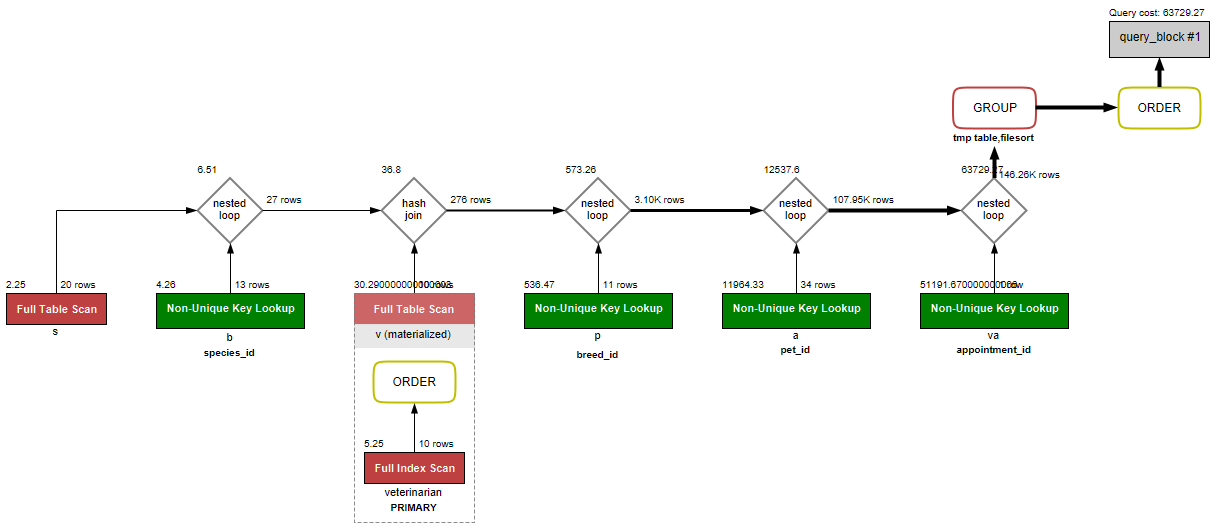
\includegraphics[width=\textwidth]{explainG8.png}
\captionsetup{justification=centering}
\caption{Графическое представление последовательности выполнения запроса 8}
\label{fig:g8}
\centering
\end{center}
\end{figure}

\subsubsection*{Гистограмма запроса}
На рис. \ref{fig:gist8} представлена 3D-гистограмма, демонстрирующая распределение приемов для каждой породы собаки и первых 10 ветеринаров.

\newpage
\begin{figure}[h!]
\begin{center}
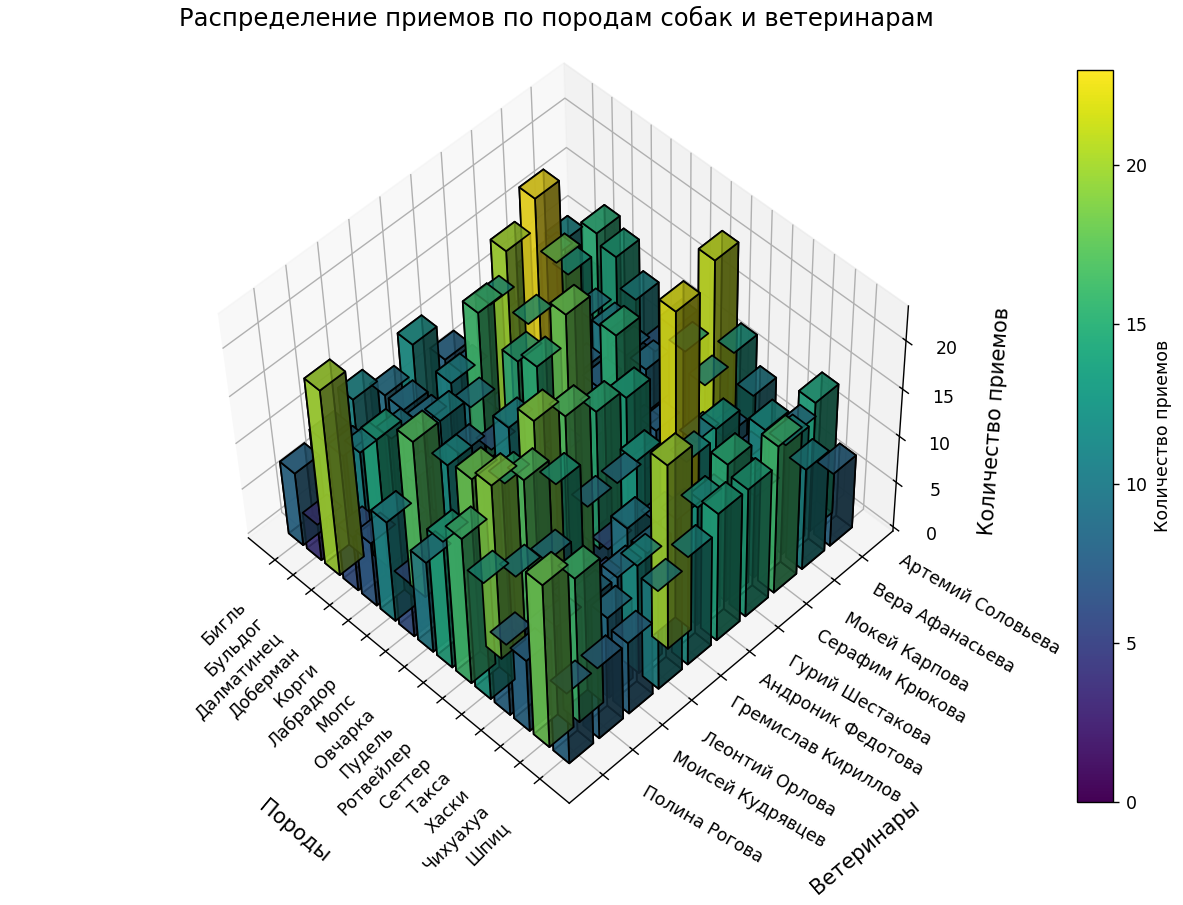
\includegraphics[width=\textwidth]{gist8.png}
\captionsetup{justification=centering}
\caption{Гистограмма запроса 8}
\label{fig:gist8}
\centering
\end{center}
\end{figure}

\newpage
\section*{Заключение}
\addcontentsline{toc}{section}{Заключение}
На первом этапе выполнения курсовой работы была выбрана и проанализирована предметная область <<Функционирование работы многопрофильной ветеринарной клиники>>. В ходе описания предметной области было выделено 7 сущностей и 37 атрибутов. На основе описанных процессов и ролей была построена ER-диаграмма, в которой количество атрибутов увеличилось до 42. Также была составлена схема связи объектов, которая содержит в себе 8 сущностей.

На втором этапе была спроектирована схема базы данных, состоящая из 12 таблиц. Для каждой таблицы были перечислены все атрибуты, их типы данных и ограничения. Для схемы базы данных было составлено графическое представление на русском и английском языках. После этого был написан код для создания базы данных и содержащихся в ней таблиц на языке MySQL в командной строке MySQL. Последним шагом база данных была заполнена 280039 записями с помощью программы, написанной на языке Python.

Третьим этапом выполнения работы является написание 8 запросов, сформированных на основе заполненной базы данных. Каждый запрос был написан на языке SQL, после чего был проанализирован с помощью команд EXPLAIN и Visual EXPLAIN.

Курсовая работа была выполнена в MySQL Workbench 8.0 CE, командной строке WINDOWS и IDLE (Python 3.12 64-bit). Работа была выполнена на ноутбуке с процессором 12th Gen Intel(R) Core(TM) i5-1235U 1.30 GHz, с 16 ГБ оперативной памяти и операционной системой Windows 11. 

\newpage
\addcontentsline{toc}{section}{Список использованных источников}
\begin{thebibliography}{9}

\bibitem{vetmed}
История ветеринарной медицины: краткий курс лекций для студентов 1 курса специальности <<Ветеринария>> / Сост.: И. Ю. Домницкий // ФГБОУ ВО Саратовский ГАУ. -- Саратов, 2016. -- 49 с. -- \href{https://www.vavilovsar.ru/files/pages/27419/14695212024.pdf?ysclid=maoj3ss533146082256}{[Электронный ресурс]} (дата обращения: 23.02.2025).

\bibitem{gost}
ГОСТ Р 55634-2013 Услуги для непродуктивных животных. Общие требования к объектам ветеринарной деятельности. -- Введ. 15-10-2013. -- М.: Стандартинформ, 2014. -- \href{https://rosgosts.ru/file/gost/03/080/gost_r_55634-2013.pdf?ysclid=maojq5zar784187663}{[Электронный ресурс]} (дата обращения: 23.02.2025).

\bibitem{civilcode}
Гражданский кодекс Российской Федерации (часть первая) от 30.11.1994 № 51-ФЗ (ред. от 21.12.2023) // КонсультантПлюс. -- \href{https://www.consultant.ru/document/cons_doc_LAW_4438/}{[Электронный ресурс]} (дата обращения: 23.02.2025).

\bibitem{pymysql}
PyMySQL Documentation / © Copyright 2023, Inada Naoki and GitHub contributors. -- URL: \url{https://pymysql.readthedocs.io/en/latest/} (дата обращения: 15.04.2025).

\bibitem{dbintro}
Введение в базы данных, 8-е издание.: Пер. с англ. -- М.: Издательский дом <<Вильяме>>, 2005. -- 1328 с.: ил. -- \href{https://psv4.userapi.com/s/v1/d/VowyPmr2QvUTLu8vP92jfnmiF3y3nCbJGZQxaINjPrzxtEkhhkR1p1rBlfDnRLGh2vle9lpvcvYZrJM-t4wVZ5nSjDBvWlmX0gNjWQLFObV18BDwNLQmRQ/Deyt_-_Vvedenie_v_sistemy_baz_dannykh.pdf}{[Электронный ресурс]}.

\end{thebibliography}

\newpage
\section*{Приложение А <<Исходный код программы генерации схемы базы данных>>}
\label{section:A}
\addcontentsline{toc}{section}{Приложение А <<Исходный код программы генерации схемы базы данных>>}
\begin{lstlisting}[basicstyle= \scriptsize \ttfamily]
CREATE DATABASE vetClinic;
USE vetClinic;

CREATE TABLE species (
    species_id INT PRIMARY KEY AUTO_INCREMENT,
    name VARCHAR(14) NOT NULL
) ENGINE=InnoDB;

CREATE TABLE breed (
    breed_id INT PRIMARY KEY AUTO_INCREMENT,
    name VARCHAR(40) NOT NULL,
    species_id INT NOT NULL,
    FOREIGN KEY (species_id) 
        REFERENCES species(species_id)
        ON DELETE CASCADE
        ON UPDATE CASCADE
) ENGINE=InnoDB;

CREATE TABLE owners (
    owner_id INT PRIMARY KEY AUTO_INCREMENT,
    first_name VARCHAR(50) NOT NULL,
    second_name VARCHAR(50) NOT NULL,
    middle_name VARCHAR(50),
    phone_number VARCHAR(20) NOT NULL,
    email VARCHAR(254),
    address VARCHAR(100)
) ENGINE=InnoDB;

CREATE TABLE pet (
    pet_id INT PRIMARY KEY AUTO_INCREMENT,
    nickname VARCHAR(50) NOT NULL,
    birth_date DATE,
    sex VARCHAR(7) NOT NULL,
    allergy VARCHAR(100),
    chip_number INT,
    owner_id INT NOT NULL,
    species_id INT NOT NULL,
    breed_id INT,
    FOREIGN KEY (owner_id) 
        REFERENCES owners(owner_id)
        ON DELETE RESTRICT
        ON UPDATE CASCADE,
    FOREIGN KEY (species_id) 
        REFERENCES species(species_id)
        ON DELETE RESTRICT
        ON UPDATE CASCADE,
    FOREIGN KEY (breed_id) 
        REFERENCES breed(breed_id)
        ON DELETE SET NULL
        ON UPDATE CASCADE
) ENGINE=InnoDB;

ALTER TABLE owners
ADD COLUMN pet_id INT NOT NULL,
ADD FOREIGN KEY (pet_id) REFERENCES pet(pet_id)
		ON DELETE CASCADE
        ON UPDATE CASCADE;

CREATE TABLE veterinarian (
    vet_id INT PRIMARY KEY AUTO_INCREMENT,
    first_name VARCHAR(50) NOT NULL,
    second_name VARCHAR(50) NOT NULL,
    middle_name VARCHAR(50),
    phone_number VARCHAR(20) NOT NULL,
    email VARCHAR(254) NOT NULL,
    specialization VARCHAR(15) NOT NULL,
    qualification VARCHAR(6) NOT NULL
) ENGINE=InnoDB;

CREATE TABLE service (
    service_id INT PRIMARY KEY AUTO_INCREMENT,
    name VARCHAR(30) NOT NULL,
    price DECIMAL(10,2) NOT NULL
) ENGINE=InnoDB;

CREATE TABLE administrator (
    admin_id INT PRIMARY KEY AUTO_INCREMENT,
    first_name VARCHAR(50) NOT NULL,
    second_name VARCHAR(50) NOT NULL,
    middle_name VARCHAR(50),
    phone_number VARCHAR(20) NOT NULL,
    email VARCHAR(254) NOT NULL
) ENGINE=InnoDB;

CREATE TABLE appointment (
    appointment_id INT PRIMARY KEY AUTO_INCREMENT,
    status VARCHAR(10) NOT NULL,
    appointment_date DATE NOT NULL,
    appointment_time TIME NOT NULL,
    reason VARCHAR(100) NOT NULL,
    conclusion VARCHAR(200),
    treatment VARCHAR(200),
    service_id INT NOT NULL,
    pet_id INT NOT NULL,
    owner_id INT NOT NULL,
    admin_id INT NOT NULL,
    FOREIGN KEY (service_id) 
        REFERENCES service(service_id)
        ON DELETE RESTRICT
        ON UPDATE CASCADE,
    FOREIGN KEY (pet_id) 
        REFERENCES pet(pet_id)
        ON DELETE RESTRICT
        ON UPDATE CASCADE,
    FOREIGN KEY (owner_id) 
        REFERENCES owners(owner_id)
        ON DELETE RESTRICT
        ON UPDATE CASCADE,
    FOREIGN KEY (admin_id) 
        REFERENCES administrator(admin_id)
        ON DELETE RESTRICT
        ON UPDATE CASCADE
) ENGINE=InnoDB;

ALTER TABLE appointment
ADD COLUMN owner_id INT NOT NULL AFTER pet_id,
ADD CONSTRAINT fk_appointment_owner
    FOREIGN KEY (owner_id)
    REFERENCES owners(owner_id)
    ON DELETE RESTRICT
    ON UPDATE CASCADE;

CREATE TABLE veterinarian_appointment (
    vet_app_id INT PRIMARY KEY AUTO_INCREMENT,
    appointment_id INT NOT NULL,
    vet_id INT NOT NULL,
    FOREIGN KEY (appointment_id) 
        REFERENCES appointment(appointment_id)
        ON DELETE CASCADE
        ON UPDATE CASCADE,
    FOREIGN KEY (vet_id) 
        REFERENCES veterinarian(vet_id)
        ON DELETE RESTRICT
        ON UPDATE CASCADE
) ENGINE=InnoDB;

CREATE TABLE supplier (
    supplier_id INT PRIMARY KEY AUTO_INCREMENT,
    name VARCHAR(50) NOT NULL
) ENGINE=InnoDB;

CREATE TABLE product (
    product_id INT PRIMARY KEY AUTO_INCREMENT,
    name VARCHAR(50) NOT NULL,
    country VARCHAR(15) NOT NULL,
    price DECIMAL(10,2) NOT NULL,
    supplier_id INT NOT NULL,
    FOREIGN KEY (supplier_id) 
        REFERENCES supplier(supplier_id)
        ON DELETE RESTRICT
        ON UPDATE CASCADE
) ENGINE=InnoDB;

CREATE TABLE purchase (
    purchase_id INT PRIMARY KEY AUTO_INCREMENT,
    purchase_date DATE NOT NULL,
    product_id INT NOT NULL,
    owner_id INT NOT NULL,
    admin_id INT NOT NULL,
    FOREIGN KEY (product_id) 
        REFERENCES Product(product_id)
        ON DELETE RESTRICT
        ON UPDATE CASCADE,
    FOREIGN KEY (owner_id) 
        REFERENCES owners(owner_id)
        ON DELETE RESTRICT
        ON UPDATE CASCADE,
    FOREIGN KEY (admin_id) 
        REFERENCES administrator(admin_id)
        ON DELETE RESTRICT
        ON UPDATE CASCADE
) ENGINE=InnoDB;
\end{lstlisting}


\newpage
\section*{Приложение Б <<Исходный код программы заполнения базы данных>>}
\label{section:Б}
\addcontentsline{toc}{section}{Приложение Б <<Исходный код программы заполения базы данных>>}
\begin{lstlisting}[caption = Подключение к базе данных, basicstyle= \scriptsize \ttfamily]
db_config = {
    'user': 'root',
    'password': 'J15ytbdaY12lh',
    'host': 'localhost',
    'database': 'vetclinic'
}
\end{lstlisting}

\begin{lstlisting}[caption = Генерация значений для таблиц, basicstyle= \scriptsize \ttfamily]
from faker import Faker
import random

fake = Faker('ru_RU')

def generate_species():
    species_list = [
        "Собака", "Кошка", "Попугай", "Хомяк", "Черепаха",
        "Кролик", "Змея", "Ящерица", "Птица", "Рыбка",
        "Морская свинка", "Крыса", "Хорёк", "Шиншилла", "Улитка",
        "Игуана", "Паук", "Хамелеон", "Песчанка", "Пони"
    ]
    return [{"name": name} for name in species_list]

BREEDS_BY_SPECIES = {
    "Собака": ["Лабрадор", "Такса", "Овчарка", "Бульдог", "Пудель", 
               "Доберман", "Ротвейлер", "Чихуахуа", "Шпиц", "Хаски",
               "Далматинец", "Бигль", "Мопс", "Корги", "Сеттер"],
    "Кошка": ["Персидская", "Сиамская", "Британская", "Мейн-кун", "Сфинкс",
              "Бенгальская", "Русская голубая", "Шотландская", "Ориентал", "Рэгдолл",
              "Бурма", "Абиссинская", "Норвежская лесная", "Сибирская", "Балинезийская"],
    "Попугай": ["Волнистый", "Корелла", "Ара", "Какаду", "Жако",
                "Неразлучник", "Розелла", "Амазон", "Ожереловый", "Лори",
                "Аратинга", "Какарик", "Сенегальский", "Эклектус", "Квакер"],
    "Хомяк": ["Джунгарский", "Сирийский", "Кэмпбелла", "Роборовский",
              "Китайский", "Эдварда", "Радеау", "Брандта", "Соболиный",
              "Жемчужный", "Коричневый", "Оранжевый", "Белый", "Золотой", "Черный"],
    "Черепаха": [ "Красноухая", "Среднеазиатская", "Болотная", "Зеленая", "Греческая",
            "Египетская", "Индийская", "Каспийская", "Мексиканская", "Леопардовая",
            "Китайский трионикс", "Мускусная", "Иловая"],
    "Кролик": [
        "Вислоухий баран", "Голландский", "Ангорский", "Рекс", "Гермелин",
        "Бабочка", "Новозеландский", "Калифорнийский", "Серебристый", "Фландр",
        "Львиноголовый", "Карликовый", "Огневка", "Бельгийский великан"
    ],
   "Змея": [
        "Королевский питон", "Молочная змея", "Кукурузная змея", "Боа констриктор",
        "Маисовый полоз", "Тигровый питон", "Радужный удав", "Уж обыкновенный",
        "Черная мамба", "Зеленая мамба", "Гадюка", "Щитомордник", "Анаконда"
    ],
    "Ящерица": [
        "Геккон", "Игуана", "Агама", "Хамелеон", "Сцинк", "Варан",
        "Анолис", "Молох", "Поясохвост", "Живородящая", "Плащеносная",
        "Водяной дракон", "Бородатая агама"
    ],
    "Птица": ["Ворон", "Дрозд", "Канарейка", "Грач", "Петух", "Снегирь",
              "Утка", "Лебедь", "Щегол", "Сова", "Голубь", "Воробей", "Синица",
              "Сойка", "Дятел"],
    "Рыбка": [
        "Гуппи", "Скалярия", "Петушок", "Меченосец", "Моллинезия",
        "Данио", "Барбус", "Неон", "Золотая рыбка", "Карп кои",
        "Дискус", "Астронотус", "Пиранья", "Арована", "Сом"
    ],
    "Морская свинка": [
        "Американская", "Абиссинская", "Перуанская", "Тексель", "Шелти",
        "Коронет", "Рекс", "Тедди", "Альпака", "Мерино", "Лункария",
        "Белая", "Трехцветная", "Гималайская"
    ],
    "Крыса": [
        "Стандарт", "Дамбо", "Рекс", "Бесхвостая", "Сфинкс", "Сатин",
        "Пуховая", "Альбинос", "Капюшон", "Беркшир", "Английская",
        "Русская голубая", "Сиамская"
    ],
    "Хорёк": [
        "Альбинос", "Соболь", "Шампань", "Корица", "Черный",
        "Белый", "Пастель", "Серебристый", "Темноглазый белый",
        "Панда", "Блейз", "Далматинец", "Шоколадный"
    ],
    "Шиншилла": [
        "Стандарт серая", "Черный бархат", "Белая", "Сапфир", "Фиолет",
        "Бежевая", "Гомобежевая", "Эбони", "Коричневая", "Гетеробежевая",
        "Пастель", "Бело-розовая", "Антрацит"
    ],
    "Улитка": [
        "Ахатина", "Виноградная", "Катушка", "Физа", "Мелания",
        "Хелена", "Мариза", "Неретина", "Ампулярия", "Теодоксус",
        "Лужанка", "Цепея", "Битиния"
    ],
    "Игуана": [
        "Зеленая", "Синяя", "Красная", "Пустынная", "Морская",
        "Чаквелла", "Анолис", "Василиск", "Шлемоносная", "Кольцехвостая",
        "Шипохвостая", "Шишковатая", "Шлемоносый василиск"
    ],
    "Паук": [
        "Птицеед", "Крестовик", "Скакун", "Волк", "Бродяга",
        "Черная вдова", "Тарантул", "Сенокосец", "Домовый",
        "Серебрянка", "Каракурт", "Бразильский странствующий",
        "Мышиный"
    ],
    "Хамелеон": [
        "Йеменский", "Пантеровый", "Джексона", "Ковровый", "Четырехрогий",
        "Малый", "Гигантский", "Фишера", "Намаква", "Брукезия",
        "Рудис", "Хохлатый", "Карликовый"
    ],
    "Песчанка": [
        "Монгольская", "Когтистая", "Индийская", "Персидская", "Сундевалла",
        "Толстохвостая", "Карликовая", "Жирнохвостая", "Короткоухая",
        "Пушистохвостая", "Белуджистанская", "Египетская", "Королевская"
    ],
    "Пони": ["Карликовый", "Золотой", "Большой", "Волнистый", "Белый",
             "В яблоко", "Серый", "Черный", "Голубой", "Пятнистый",
             "Полосатый", "Пушистый", "Китайский", "Японский", "Коричневый"]
}

def generate_breeds(species_list):
    breeds = []
    for species in species_list:
        species_name = species["name"]
        species_id = species["species_id"]
        for breed_name in random.sample(BREEDS_BY_SPECIES.get(species_name, []), 
                                      min(15, len(BREEDS_BY_SPECIES.get(species_name, [])))):
            breeds.append({
                "name": breed_name,
                "species_id": species_id
            })
    return breeds

def generate_suppliers(count=50):
    suppliers = []
    for _ in range(count):
        suppliers.append({
            'name': fake.company()  
        })
    return suppliers

def generate_veterinarians(count=50):
    veterinarians = []
    specializations = [
        'Хирург', 'Терапевт', 'Офтальмолог', 'Дерматолог', 
        'Кардиолог', 'Невролог', 'Онколог', 'Стоматолог',
        'Уролог', 'Лаборант'
    ]
    qualifications = ['Высшая', 'Первая', 'Вторая']
    
    for _ in range(count):
        veterinarians.append({
            'first_name': fake.first_name_male() if random.choice([True, False]) else fake.first_name_female(),
            'second_name': fake.last_name_male() if random.choice([True, False]) else fake.last_name_female(),
            'middle_name': fake.middle_name_male() if random.choice([True, False]) else fake.middle_name_female(),
            'phone_number': fake.phone_number(),
            'email': fake.email(),
            'specialization': random.choice(specializations),
            'qualification': random.choice(qualifications)
        })
    return veterinarians

def generate_administrators(count=50):
    administrators = []
    for _ in range(count):
        gender = random.choice(['male', 'female'])
        administrators.append({
            'first_name': fake.first_name_male() if gender == 'male' else fake.first_name_female(),
            'second_name': fake.last_name_male() if gender == 'male' else fake.last_name_female(),
            'middle_name': fake.middle_name_male() if gender == 'male' else fake.middle_name_female(),
            'phone_number': f"+7({fake.random_int(900, 999)}){fake.random_int(100, 999)}-{fake.random_int(10, 99)}-{fake.random_int(10, 99)}",
            'email': f"{fake.user_name()}{fake.random_int(1, 99)}@{fake.domain_name()}"
        })
    return administrators


def generate_services():
    services = [
        {"name": "Первичный осмотр", "price": 1500.00},
        {"name": "Повторный осмотр", "price": 1000.00},
        {"name": "Вакцинация", "price": 2000.00},
        {"name": "Чипирование", "price": 2500.00},
        {"name": "Кастрация кота", "price": 5000.00},
        {"name": "Стерилизация кошки", "price": 8000.00},
        {"name": "УЗИ брюшной полости", "price": 3500.00},
        {"name": "Рентген", "price": 3000.00},
        {"name": "Анализ крови", "price": 2500.00},
        {"name": "Чистка зубов", "price": 4000.00},
        {"name": "Удаление зубов", "price": 6000.00},
        {"name": "Обработка от паразитов", "price": 1800.00},
        {"name": "Подстригание когтей", "price": 800.00},
        {"name": "Перевязка", "price": 1200.00},
        {"name": "Наложение швов", "price": 3500.00},
        {"name": "Капельница", "price": 2000.00},
        {"name": "Госпитализация (сутки)", "price": 4500.00},
        {"name": "ЭКГ", "price": 2800.00},
        {"name": "Анализ мочи", "price": 1500.00},
        {"name": "Анализ кала", "price": 1700.00},
        {"name": "Тримминг", "price": 2500.00},
        {"name": "Груминг мелких пород", "price": 3500.00},
        {"name": "Груминг средних пород", "price": 4500.00},
        {"name": "Груминг крупных пород", "price": 6000.00},
        {"name": "Вызов на дом", "price": 3000.00},
        {"name": "Эвтаназия", "price": 4000.00},
        {"name": "Кремация", "price": 7000.00},
        {"name": "Скорая помощь", "price": 5000.00},
        {"name": "Консультация диетолога", "price": 2500.00},
        {"name": "Консультация хирурга", "price": 3000.00},
        {"name": "Консультация онколога", "price": 3500.00},
        {"name": "Физиотерапия", "price": 2800.00},
        {"name": "Лазерная терапия", "price": 3200.00},
        {"name": "Химиотерапия", "price": 8500.00},
        {"name": "Онкологическая операция", "price": 15000.00},
        {"name": "Офтальмологический осмотр", "price": 2200.00},
        {"name": "Стоматологический осмотр", "price": 1800.00},
        {"name": "Дерматологический осмотр", "price": 2000.00},
        {"name": "Кардиологический осмотр", "price": 3500.00},
        {"name": "Неврологический осмотр", "price": 3800.00},
        {"name": "Ортопедический осмотр", "price": 3000.00},
        {"name": "Родыспоможение", "price": 10000.00},
        {"name": "Кесарево сечение", "price": 12000.00},
        {"name": "Микроскопия кожи", "price": 1800.00},
        {"name": "Цитологическое исследование", "price": 2500.00},
        {"name": "Гистологическое исследование", "price": 5000.00},
        {"name": "Анестезия", "price": 3000.00},
        {"name": "Реанимационные мероприятия", "price": 6000.00},
        {"name": "Интенсивная терапия", "price": 4500.00},
        {"name": "Переливание крови", "price": 8000.00}
    ]
    return services

def generate_products(supplier_ids, count=700):
    products = []
    categories = {
        'Корм': ['сухой', 'влажный', 'консервы', 'премиум', 'холистик'],
        'Лекарства': ['антибиотики', 'витамины', 'противопаразитарные', 'анальгетики', 'противовоспалительные'],
        'Аксессуары': ['ошейники', 'поводки', 'миски', 'лежанки', 'переноски'],
        'Гигиена': ['шампуни', 'расчески', 'зубные щетки', 'пеленки', 'салфетки'],
        'Игрушки': ['мячи', 'пищалки', 'интерактивные', 'канаты', 'грызунки']
    }
    
    countries = ['Россия', 'Германия', 'Франция', 'США', 'Великобритания', 'Китай', 'Италия', 'Испания']

    supplier_cycle = supplier_ids * (count // len(supplier_ids))
    remaining = count % len(supplier_ids)
    supplier_cycle += supplier_ids[:remaining]
    
    for _ in range(count):
        category = random.choice(list(categories.keys()))
        subcategory = random.choice(categories[category])
        products.append({
            'name': f"{category} {subcategory} {fake.word()}",
            'country': random.choice(countries),
            'price': round(random.uniform(50, 5000), 2),
            'supplier_id': random.choice(supplier_ids)
        })
    return products

def generate_owners(count=200):
    owners = []
    for _ in range(count):
        gender = random.choice(['male', 'female'])
        owners.append({
            'first_name': fake.first_name_male() if gender == 'male' else fake.first_name_female(),
            'second_name': fake.last_name_male() if gender == 'male' else fake.last_name_female(),
            'middle_name': fake.middle_name_male() if gender == 'male' else fake.middle_name_female(),
            'phone_number': f"+7({fake.random_int(900, 999)}){fake.random_int(100, 999)}-{fake.random_int(10, 99)}-{fake.random_int(10, 99)}",
            'email': f"{fake.user_name()}{random.randint(1, 99)}@{fake.domain_name()}",
            'address': f"{fake.city()}, ул. {fake.street_name()}, д. {fake.building_number()}"
        })
    return owners

def generate_pets(owner_ids, species_list, breed_list, pets_per_owner=(1, 30)):
    pets = []
    pet_names = {
        'Собака': ['Шарик', 'Рекс', 'Джек', 'Белка', 'Тузик', 'Лорд', 'Цезарь', 
                  'Бобик', 'Ральф', 'Арчи', 'Граф', 'Дейзи', 'Лайма', 'Зевс', 'Оскар', 'Чарли', 'Тедди'],
        'Кошка': ['Мурзик', 'Васька', 'Пушистик', 'Снежок', 'Рыжик', 'Персик', 'Барсик', 'Мурка',
                 'Симба', 'Луна', 'Оливер', 'Лео', 'Мия', 'Тигра', 'Сэм', 'Люси', 'Гарфилд', 'Нюша'],
        'Попугай': ['Кеша', 'Гоша', 'Рио', 'Арчи', 'Яша', 'Кира', 'Лора', 'Чижик',
                   'Коко', 'Жак', 'Пип', 'Рики', 'Чико', 'Бонни', 'Клео', 'Лори'],
        'Хомяк': ['Пушок', 'Нюша', 'Боня', 'Фунтик', 'Пиксель', 'Кнопа', 'Сеня', 'Зефирка',
                 'Хома', 'Буся', 'Мотя', 'Кругляш', 'Цуки', 'Филя', 'Шуша', 'Плюша'],
        'Черепаха': ['Тоша', 'Шелл', 'Донни', 'Лео', 'Рафа', 'Мики', 'Сплинтер', 'Вальт',
                    'Спиди', 'Касси', 'Тортилла', 'Бабблз', 'Шелдон', 'Квази', 'Танк'],
        'Кролик': ['Роджер', 'Багз', 'Лола', 'Снежок', 'Пухля', 'Флаффи', 'Банни', 'Джаспер',
                  'Орео', 'Коко', 'Питер', 'Дейзи', 'Макс', 'Лулу', 'Симба'],
        'Змея': ['Нага', 'Каа', 'Зигги', 'Сайрен', 'Пайтон', 'Медяна', 'Слизи', 'Вайпер',
                'Барон', 'Гиза', 'Спаркл', 'Эсмеральда', 'Оникс', 'Салазар'],
        'Ящерица': ['Годзилла', 'Иго', 'Рекс', 'Спайк', 'Дарт', 'Скала', 'Зилла', 'Гекко',
                   'Риптор', 'Драко', 'Твигги', 'Йоши', 'Комодо', 'Сцинк'],
        'Птица': ['Квизи', 'Твити', 'Блю', 'Скай', 'Санни', 'Пип', 'Чип', 'Дейзи',
                 'Рио', 'Альба', 'Перси', 'Спарки', 'Феникс', 'Валькирия'],
        'Рыбка': ['Немо', 'Дори', 'Баббл', 'Голди', 'Флиппер', 'Спот', 'Близзард', 'Неон',
                 'Азур', 'Коралл', 'Плавник', 'Жабр', 'Скаляр', 'Гуппи'],
        'Морская свинка': ['Пигги', 'Гвинни', 'Флафф', 'Сквик', 'Бекон', 'Панкейк', 'Мох', 'Пух',
                          'Шоколад', 'Карамель', 'Пончик', 'Бисквит', 'Пельмень', 'Вафля'],
        'Крыса': ['Рэтчет', 'Рэтту', 'Сквиджи', 'Твич', 'Сникерс', 'Пипсквик', 'Гном', 'Шашлык',
                 'Рокки', 'Скраффи', 'Чиззи', 'Рэттиган', 'Сплinter', 'Тайл'],
        'Хорёк': ['Фредди', 'Ферби', 'Ласка', 'Джинкс', 'Зип', 'Слим', 'Виззи', 'Фуззи',
                'Нудл', 'Сквирт', 'Фигаро', 'Локи', 'Пикси', 'Твинкл'],
        'Шиншилла': ['Чилла', 'Душка', 'Плюш', 'Шани', 'Чоко', 'Латте', 'Марш', 'Зефир',
                    'Бамбино', 'Чиби', 'Пуфик', 'Сноу', 'Мисти', 'Эльф'],
        'Улитка': ['Турбо', 'Шелл', 'Спиди', 'Слизз', 'Баббл', 'Гэри', 'Эскарго', 'Сникер',
                  'Крулл', 'Спираль', 'Койл', 'Слимп', 'Густо', 'Баблз'],
        'Игуана': ['Изи', 'Годзи', 'Спайк', 'Зилла', 'Рекс', 'Драгон', 'Торч', 'Смауг',
                  'Риптор', 'Скала', 'Огненный', 'Альберт', 'Кома', 'Зорро'],
        'Паук': ['Питер', 'Шелоб', 'Арахна', 'Веном', 'Тара', 'Фанг', 'Чарли', 'Скай',
                'Октобер', 'Инки', 'Спайдер', 'Уиджи', 'Локи', 'Зорг'],
        'Хамелеон': ['Камео', 'Рэйнбоу', 'Зигги', 'Лео', 'Джаспер', 'Рипли', 'Пантер', 'Мистик',
                    'Сэм', 'Блендер', 'Краска', 'Халк', 'Ирис', 'Клевер'],
        'Песчанка': ['Джерри', 'Санд', 'Джинжер', 'Ниббл', 'Скутер', 'Пип', 'Твич', 'Джампер',
                    'Бисквит', 'Флик', 'Зип', 'Спарки', 'Флип', 'Бамбл'],
        'Пони': ['Пинки', 'Твай', 'Рарити', 'Эпл', 'Флаттер', 'Спайк', 'Скут', 'Каденс',
               'Санни', 'Луна', 'Стар', 'Шугар', 'Баттер', 'Блу']
    }
    
    used_chip_numbers = set()
    owner_pet_counts = {owner_id: random.randint(*pets_per_owner) for owner_id in owner_ids}
    
    for owner_id, pet_count in owner_pet_counts.items():
        for _ in range(pet_count):
            species = random.choice(species_list)
            species_id = species['species_id']
            species_name = species['name']
            
            available_breeds = [b for b in breed_list if b['species_id'] == species_id]
            breed = random.choice(available_breeds) if available_breeds else None

            chip = None
            if random.random() > 0.7:
                while True:
                    new_chip = random.randint(100000000, 2147483647)
                    if new_chip not in used_chip_numbers:
                        used_chip_numbers.add(new_chip)
                        chip = new_chip
                        break
            
            name_options = pet_names.get(species_name, ['Дружок', 'Счастливчик', 'Лапуля'])
            
            pets.append({
                'nickname': random.choice(name_options),
                'birth_date': fake.date_between(start_date='-15y', end_date='-1y').strftime('%Y-%m-%d'),
                'sex': random.choice(['Male', 'Female']),
                'allergy': random.choice([None, 'Пыльца', 'Курица', 'Злаки', 'Блошиный укус']),
                'chip_number': chip,
                'owner_id': owner_id,
                'species_id': species_id,
                'breed_id': breed['breed_id'] if breed else None })
    
    return pets

def generate_purchases(owner_ids, product_ids, admin_ids, purchases_per_owner=(40, 80)):
    purchases = []
    owner_purchase_counts = {owner_id: random.randint(*purchases_per_owner) for owner_id in owner_ids}
    total_purchases = sum(owner_purchase_counts.values())

    admin_pool = []

    base_per_admin = max(1, total_purchases // len(admin_ids) - 10)
    for admin_id in admin_ids:
        admin_pool.extend([admin_id] * base_per_admin)

    remaining = total_purchases - len(admin_pool)
    if remaining > 0:
        extra_admins = random.choices(admin_ids, k=remaining)
        admin_pool.extend(extra_admins)
    random.shuffle(admin_pool)  

    product_weights = [random.uniform(0.3, 1.7) for _ in product_ids]  # Разная популярность
    product_pool = random.choices(
        product_ids, 
        weights=product_weights,
        k=total_purchases
    )
    purchase_index = 0
    for owner_id, purchase_count in owner_purchase_counts.items():
        for _ in range(purchase_count):
            purchases.append({
                'purchase_date': fake.date_between(start_date='-2y', end_date='today').strftime('%Y-%m-%d'),
                'product_id': product_pool[purchase_index],
                'owner_id': owner_id,
                'admin_id': admin_pool[purchase_index]
            })
            purchase_index += 1
    
    return purchases

def generate_appointments(pet_list, service_ids, admin_ids, appointments_per_pet=(20, 50)):
    appointments = []
    reasons = [
        "Плановый осмотр", "Вакцинация", "Травма", 
        "Кожные проблемы", "Проблемы с ЖКТ", "Стоматология",
        "Аллергия", "Кастрация/стерилизация", "Чипирование"
    ]
    treatments = [
        "Назначены лекарства", "Рекомендован отдых", 
        "Проведена операция", "Назначена диета",
        "Рекомендованы дополнительные анализы", "Проведена обработка"
    ]
    conclusions = [
        "Здоров", "Требуется наблюдение", "Хроническое заболевание",
        "Острое состояние", "Послеоперационный уход", "Ремиссия"
    ]
    pet_appointment_counts = {pet['pet_id']: random.randint(*appointments_per_pet) for pet in pet_list}
    total_appointments = sum(pet_appointment_counts.values())
    
    admin_appointment_counts = {}
    remaining = total_appointments
    num_admins = len(admin_ids)
    
    for i, admin_id in enumerate(admin_ids[:-1]):
        min_a = max(20, remaining - 50 * (num_admins - i - 1))
        max_a = min(50, remaining - 20 * (num_admins - i - 1))
        if min_a > max_a:
            count = (min_a + max_a) // 2
        else:
            count = random.randint(min_a, max_a)
            
        admin_appointment_counts[admin_id] = count
        remaining -= count

    admin_appointment_counts[admin_ids[-1]] = remaining

    admin_pool = []
    for admin_id, count in admin_appointment_counts.items():
        admin_pool.extend([admin_id] * count)
    random.shuffle(admin_pool)
    
    appointment_index = 0
    for pet in pet_list:
        pet_id = pet['pet_id']
        owner_id = pet['owner_id']
        pet_services = [random.choice(service_ids) for _ in range(pet_appointment_counts[pet_id])]
        for service_id in pet_services:
            appointment_date = fake.date_between(start_date='-2y', end_date='today')
            appointments.append({
                'status': random.choice(['Completed', 'Cancelled', 'No-show']),
                'appointment_date': appointment_date.strftime('%Y-%m-%d'),
                'appointment_time': fake.time(pattern='%H:%M'),
                'reason': random.choice(reasons),
                'conclusion': random.choice(conclusions) if random.random() > 0.2 else None,
                'treatment': random.choice(treatments) if random.random() > 0.3 else None,
                'service_id': service_id,
                'pet_id': pet_id,
                'owner_id': owner_id,
                'admin_id': admin_pool[appointment_index]
            })
            appointment_index += 1
    return appointments

def generate_vet_appointments(appointment_ids, vet_ids):
    vet_appointments = []
    vet_cycle = (vet_ids * ((len(appointment_ids) // len(vet_ids)) + 1))[:len(appointment_ids)]
    for i, appointment_id in enumerate(appointment_ids):
        vet_appointments.append({
            'appointment_id': appointment_id,
            'vet_id': vet_cycle[i]
        })
        if random.random() < 0.3:
            additional_vets = random.sample(vet_ids, random.randint(1, 2))
            for vet_id in additional_vets:
                if vet_id != vet_cycle[i]:  
                    vet_appointments.append({
                        'appointment_id': appointment_id,
                        'vet_id': vet_id
                    })
    return vet_appointments
\end{lstlisting}

\begin{lstlisting}[caption = Заполнение таблицы Species, basicstyle= \scriptsize \ttfamily]
import mysql.connector
from config import db_config
from fake_data import generate_species

def fill_species():
    species = generate_species() 
    conn = mysql.connector.connect(**db_config)
    cursor = conn.cursor()

    for item in species:
        cursor.execute(
            "INSERT INTO species (name) VALUES (%s)",
            (item["name"],)
        )
    
    conn.commit()
    cursor.close()
    conn.close()
    print(f"Добавлено {len(species)} записей в таблицу species!")

if __name__ == "__main__":
    fill_species()
\end{lstlisting}

\begin{lstlisting}[caption = Заполнение таблицы Breed, basicstyle= \scriptsize \ttfamily]
import mysql.connector
from config import db_config
from fake_data import generate_species
from fake_data import generate_breeds

def get_existing_species(conn):
    cursor = conn.cursor()
    cursor.execute("SELECT species_id, name FROM species")
    species_list = [{"species_id": row[0], "name": row[1]} for row in cursor.fetchall()]
    cursor.close()
    return species_list

def fill_breed():
    conn = mysql.connector.connect(**db_config)

    species_list = get_existing_species(conn)

    breeds = generate_breeds(species_list)

    cursor = conn.cursor()
    for breed in breeds:
        cursor.execute(
            "INSERT INTO breed (name, species_id) VALUES (%s, %s)",
            (breed["name"], breed["species_id"])
        )
    
    conn.commit()
    cursor.close()
    conn.close()
    print(f"Добавлено {len(breeds)} записей в таблицу breed!")

if __name__ == "__main__":
    fill_breed()
\end{lstlisting}

\begin{lstlisting}[caption = Заполнение таблицы Owners, basicstyle= \scriptsize \ttfamily]
import mysql.connector
from config import db_config
from fake_data import generate_owners

def fill_owners():
    conn = mysql.connector.connect(**db_config)
    cursor = conn.cursor()

    cursor.execute("SET FOREIGN_KEY_CHECKS = 0")
    cursor.execute("TRUNCATE TABLE owners")
    cursor.execute("ALTER TABLE owners AUTO_INCREMENT = 1")
    cursor.execute("SET FOREIGN_KEY_CHECKS = 1")
    
    owners = generate_owners(200)
    for owner in owners:
        cursor.execute(
            """INSERT INTO owners 
            (first_name, second_name, middle_name, phone_number, email, address)
            VALUES (%s, %s, %s, %s, %s, %s)""",
            (owner['first_name'], owner['second_name'], owner['middle_name'],
             owner['phone_number'], owner['email'], owner['address'])
        )
    
    conn.commit()
    cursor.close()
    conn.close()
    print(f"Добавлено {len(owners)} владельцев!")

if __name__ == "__main__":
    fill_owners()
\end{lstlisting}

\begin{lstlisting}[caption = Заполнение таблицы Pet, basicstyle= \scriptsize \ttfamily]
import mysql.connector
from config import db_config
from fake_data import generate_pets

def get_owner_ids(conn):
    cursor = conn.cursor(dictionary=True)
    cursor.execute("SELECT owner_id FROM owners")
    return [row['owner_id'] for row in cursor.fetchall()]

def get_species_list(conn):
    cursor = conn.cursor(dictionary=True)
    cursor.execute("SELECT species_id, name FROM species")
    return cursor.fetchall()

def get_breed_list(conn):
    cursor = conn.cursor(dictionary=True)
    cursor.execute("SELECT breed_id, species_id FROM breed")
    return cursor.fetchall()

def fill_pets():
    conn = mysql.connector.connect(**db_config)
    cursor = conn.cursor()
    
    try:
        cursor.execute("SET FOREIGN_KEY_CHECKS = 0")
        cursor.execute("TRUNCATE TABLE pet")
        cursor.execute("ALTER TABLE pet AUTO_INCREMENT = 1")
        cursor.execute("SET FOREIGN_KEY_CHECKS = 1")

        owner_ids = get_owner_ids(conn)
        species_list = get_species_list(conn)
        breed_list = get_breed_list(conn)

        pets = generate_pets(owner_ids, species_list, breed_list)
        
        for pet in pets:
            cursor.execute(
                """INSERT INTO pet 
                (nickname, birth_date, sex, allergy, chip_number, owner_id, species_id, breed_id)
                VALUES (%s, %s, %s, %s, %s, %s, %s, %s)""",
                (pet['nickname'], pet['birth_date'], pet['sex'], pet['allergy'],
                 pet['chip_number'], pet['owner_id'], pet['species_id'], pet['breed_id'])
            )
        
        conn.commit()
        print(f"Добавлено {len(pets)} питомцев!")

if __name__ == "__main__":
    fill_pets()
\end{lstlisting}

\begin{lstlisting}[caption = Заполнение таблицы Service, basicstyle= \scriptsize \ttfamily]
import mysql.connector
from config import db_config
from fake_data import generate_services

def fill_services():
    conn = mysql.connector.connect(**db_config)
    cursor = conn.cursor()

    cursor.execute("SET FOREIGN_KEY_CHECKS = 0")
    cursor.execute("TRUNCATE TABLE service")
    cursor.execute("ALTER TABLE service AUTO_INCREMENT = 1")
    cursor.execute("SET FOREIGN_KEY_CHECKS = 1")

    services = generate_services()
    for service in services:
        cursor.execute(
            """INSERT INTO service 
            (name, price)
            VALUES (%s, %s)""",
            (service['name'], service['price'])
        )
    
    conn.commit()
    cursor.close()
    conn.close()
    print(f"Добавлено {len(services)} услуг!")

if __name__ == "__main__":
    fill_services()
\end{lstlisting}

\begin{lstlisting}[caption = Заполнение таблицы Administrator, basicstyle= \scriptsize \ttfamily]
import mysql.connector
from config import db_config
from fake_data import generate_administrators

def fill_administrators():
    conn = mysql.connector.connect(**db_config)
    cursor = conn.cursor()

    cursor.execute("SET FOREIGN_KEY_CHECKS = 0")
    cursor.execute("TRUNCATE TABLE administrator")
    cursor.execute("ALTER TABLE administrator AUTO_INCREMENT = 1")
    cursor.execute("SET FOREIGN_KEY_CHECKS = 1")

    admins = generate_administrators(50)
    for admin in admins:
        cursor.execute(
            """INSERT INTO administrator 
            (first_name, second_name, middle_name, phone_number, email)
            VALUES (%s, %s, %s, %s, %s)""",
            (admin['first_name'], admin['second_name'], admin['middle_name'],
             admin['phone_number'], admin['email'])
        )
    
    conn.commit()
    cursor.close()
    conn.close()
    print(f"Добавлено {len(admins)} администраторов!")

if __name__ == "__main__":
    fill_administrators()
\end{lstlisting}

\begin{lstlisting}[caption = Заполнение таблицы Appointment, basicstyle= \scriptsize \ttfamily]
import mysql.connector
from config import db_config
from fake_data import generate_appointments

def get_pet_list(conn):
    cursor = conn.cursor(dictionary=True)
    cursor.execute("SELECT pet_id, owner_id FROM pet")
    return cursor.fetchall()

def get_service_ids(conn):
    cursor = conn.cursor()
    cursor.execute("SELECT service_id FROM service")
    return [row[0] for row in cursor.fetchall()]

def get_admin_ids(conn):
    cursor = conn.cursor()
    cursor.execute("SELECT admin_id FROM administrator")
    return [row[0] for row in cursor.fetchall()]

def fill_appointments():
    conn = mysql.connector.connect(**db_config)
    cursor = conn.cursor()
    
    try:
        cursor.execute("SET FOREIGN_KEY_CHECKS = 0")
        cursor.execute("TRUNCATE TABLE appointment")
        cursor.execute("ALTER TABLE appointment AUTO_INCREMENT = 1")
        cursor.execute("SET FOREIGN_KEY_CHECKS = 1")
        
        pet_list = get_pet_list(conn)
        service_ids = get_service_ids(conn)
        admin_ids = get_admin_ids(conn)

        appointments = generate_appointments(pet_list, service_ids, admin_ids)
        
        for appointment in appointments:
            cursor.execute(
                """INSERT INTO appointment 
                (status, appointment_date, appointment_time, reason, 
                 conclusion, treatment, service_id, pet_id, owner_id, admin_id)
                VALUES (%s, %s, %s, %s, %s, %s, %s, %s, %s, %s)""",
                (appointment['status'], appointment['appointment_date'],
                 appointment['appointment_time'], appointment['reason'],
                 appointment['conclusion'], appointment['treatment'],
                 appointment['service_id'], appointment['pet_id'],
                 appointment['owner_id'], appointment['admin_id'])
            )
        
        conn.commit()
        print(f"Добавлено {len(appointments)} приемов!")

if __name__ == "__main__":
    fill_appointments()
\end{lstlisting}

\begin{lstlisting}[caption = Заполнение таблицы Veterinarian, basicstyle= \scriptsize \ttfamily]
import mysql.connector
from config import db_config
from fake_data import generate_veterinarians

def fill_veterinarians():
    conn = mysql.connector.connect(**db_config)
    cursor = conn.cursor()

    cursor.execute("SET FOREIGN_KEY_CHECKS = 0")
    cursor.execute("TRUNCATE TABLE veterinarian")
    cursor.execute("ALTER TABLE veterinarian AUTO_INCREMENT = 1")
    cursor.execute("SET FOREIGN_KEY_CHECKS = 1")

    vets = generate_veterinarians(50)
    for vet in vets:
        cursor.execute(
            """INSERT INTO veterinarian 
            (first_name, second_name, middle_name, phone_number, email, specialization, qualification)
            VALUES (%s, %s, %s, %s, %s, %s, %s)""",
            (vet['first_name'], vet['second_name'], vet['middle_name'], 
             vet['phone_number'], vet['email'], vet['specialization'], vet['qualification'])
        )
    conn.commit()
    cursor.close()
    conn.close()
    print(f"Добавлено {len(vets)} ветеринаров!")

if __name__ == "__main__":
    fill_veterinarians()
\end{lstlisting}

\begin{lstlisting}[caption = Заполнение таблицы Veterinarian and appointment, basicstyle= \scriptsize \ttfamily]
import mysql.connector
from config import db_config
from fake_data import generate_vet_appointments

def get_appointment_ids(conn):
    cursor = conn.cursor()
    cursor.execute("SELECT appointment_id FROM appointment")
    return [row[0] for row in cursor.fetchall()]

def get_vet_ids(conn):
    cursor = conn.cursor()
    cursor.execute("SELECT vet_id FROM veterinarian")
    return [row[0] for row in cursor.fetchall()]

def fill_vet_appointments():
    conn = mysql.connector.connect(**db_config)
    cursor = conn.cursor()
    
    try:
        cursor.execute("SET FOREIGN_KEY_CHECKS = 0")
        cursor.execute("TRUNCATE TABLE veterinarian_appointment")
        cursor.execute("ALTER TABLE veterinarian_appointment AUTO_INCREMENT = 1")
        cursor.execute("SET FOREIGN_KEY_CHECKS = 1")

        appointment_ids = get_appointment_ids(conn)
        vet_ids = get_vet_ids(conn)

        vet_appointments = generate_vet_appointments(appointment_ids, vet_ids)
        
        for va in vet_appointments:
            cursor.execute(
                """INSERT INTO veterinarian_appointment 
                (appointment_id, vet_id)
                VALUES (%s, %s)""",
                (va['appointment_id'], va['vet_id'])
            )
        
        conn.commit()
        print(f"Добавлено {len(vet_appointments)} связей ветеринаров с приемами!")

if __name__ == "__main__":
    fill_vet_appointments()
\end{lstlisting}

\begin{lstlisting}[caption = Заполнение таблицы Supplier, basicstyle= \scriptsize \ttfamily]
import mysql.connector
from config import db_config
from fake_data import generate_suppliers

def fill_suppliers():
    suppliers = generate_suppliers(50)
    conn = mysql.connector.connect(**db_config)
    cursor = conn.cursor()

    for supplier in suppliers:
        cursor.execute(
            "INSERT INTO supplier (name) VALUES (%s)",
            (supplier['name'],)
        )
    
    conn.commit()
    cursor.close()
    conn.close()
    print(f"Добавлено {len(suppliers)} поставщиков!")

if __name__ == "__main__":
    fill_suppliers()
\end{lstlisting}

\begin{lstlisting}[caption = Заполнение таблицы Product, basicstyle= \scriptsize \ttfamily]
import mysql.connector
import random
from config import db_config
from fake_data import generate_products

def get_supplier_ids(conn):
    cursor = conn.cursor()
    cursor.execute("SELECT supplier_id FROM supplier")
    supplier_ids = [row[0] for row in cursor.fetchall()]
    cursor.close()
    return supplier_ids

def fill_products():
    conn = mysql.connector.connect(**db_config)
    cursor = conn.cursor()

    cursor.execute("SET FOREIGN_KEY_CHECKS = 0")
    cursor.execute("TRUNCATE TABLE product")
    cursor.execute("ALTER TABLE product AUTO_INCREMENT = 1")
    cursor.execute("SET FOREIGN_KEY_CHECKS = 1")

    supplier_ids = get_supplier_ids(conn)

    products = generate_products(supplier_ids, 700)
    for product in products:
        cursor.execute(
            """INSERT INTO product 
            (name, country, price, supplier_id)
            VALUES (%s, %s, %s, %s)""",
            (product['name'], product['country'], 
             product['price'], product['supplier_id'])
        )
    
    conn.commit()
    cursor.close()
    conn.close()
    print(f"Добавлено {len(products)} товаров!")

if __name__ == "__main__":
    fill_products()

\end{lstlisting}

\begin{lstlisting}[caption = Заполнение таблицы Purchase, basicstyle= \scriptsize \ttfamily]
import mysql.connector
from config import db_config
from fake_data import generate_purchases

def get_owner_ids(conn):
    cursor = conn.cursor()
    cursor.execute("SELECT owner_id FROM owners")
    return [row[0] for row in cursor.fetchall()]

def get_product_ids(conn):
    cursor = conn.cursor()
    cursor.execute("SELECT product_id FROM product")
    return [row[0] for row in cursor.fetchall()]

def get_admin_ids(conn):
    cursor = conn.cursor()
    cursor.execute("SELECT admin_id FROM administrator")
    return [row[0] for row in cursor.fetchall()]

def fill_purchases():
    conn = mysql.connector.connect(**db_config)
    cursor = conn.cursor()
    
    try:
        cursor.execute("SET FOREIGN_KEY_CHECKS = 0")
        cursor.execute("TRUNCATE TABLE purchase")
        cursor.execute("ALTER TABLE purchase AUTO_INCREMENT = 1")
        cursor.execute("SET FOREIGN_KEY_CHECKS = 1")

        owner_ids = get_owner_ids(conn)
        product_ids = get_product_ids(conn)
        admin_ids = get_admin_ids(conn)

        purchases = generate_purchases(owner_ids, product_ids, admin_ids)
        
        for purchase in purchases:
            cursor.execute(
                """INSERT INTO purchase 
                (purchase_date, product_id, owner_id, admin_id)
                VALUES (%s, %s, %s, %s)""",
                (purchase['purchase_date'], purchase['product_id'], 
                 purchase['owner_id'], purchase['admin_id'])
            )
        
        conn.commit()
        print(f"Добавлено {len(purchases)} покупок!")

if __name__ == "__main__":
    fill_purchases()
\end{lstlisting}

\end{document}
